
\newpage
\section{Example Results}

This section presents example results for different configurations of the Orthogonal Vector Visualization System. It shows the generated vectors and their visualizations for various parameter values.

\subsection{Single Vector Generation}

The system generates a single R vector using scalar formulas. The default configuration uses the origin [0, 0, 0] with a distance parameter of 1.0 and an angle parameter of $\pi/4$.

\subsubsection{Scalar Formulation}

The R vector is calculated using the following scalar formula:

\begin{align}
\vec{R} = \vec{R}_0 + d \cdot \cos(\theta) \cdot \sqrt{\frac{2}{3}} + d \cdot \frac{\cos(\theta)/\sqrt{3} + \sin(\theta)}{\sqrt{2}} + d \cdot \frac{\sin(\theta) - \cos(\theta)/\sqrt{3}}{\sqrt{2}} - 2 \cdot \vec{R}_0
\end{align}

This formula combines three orthogonal components to produce a single resulting vector.

\subsubsection{3D Visualization}

\begin{figure}[H]
    \centering
    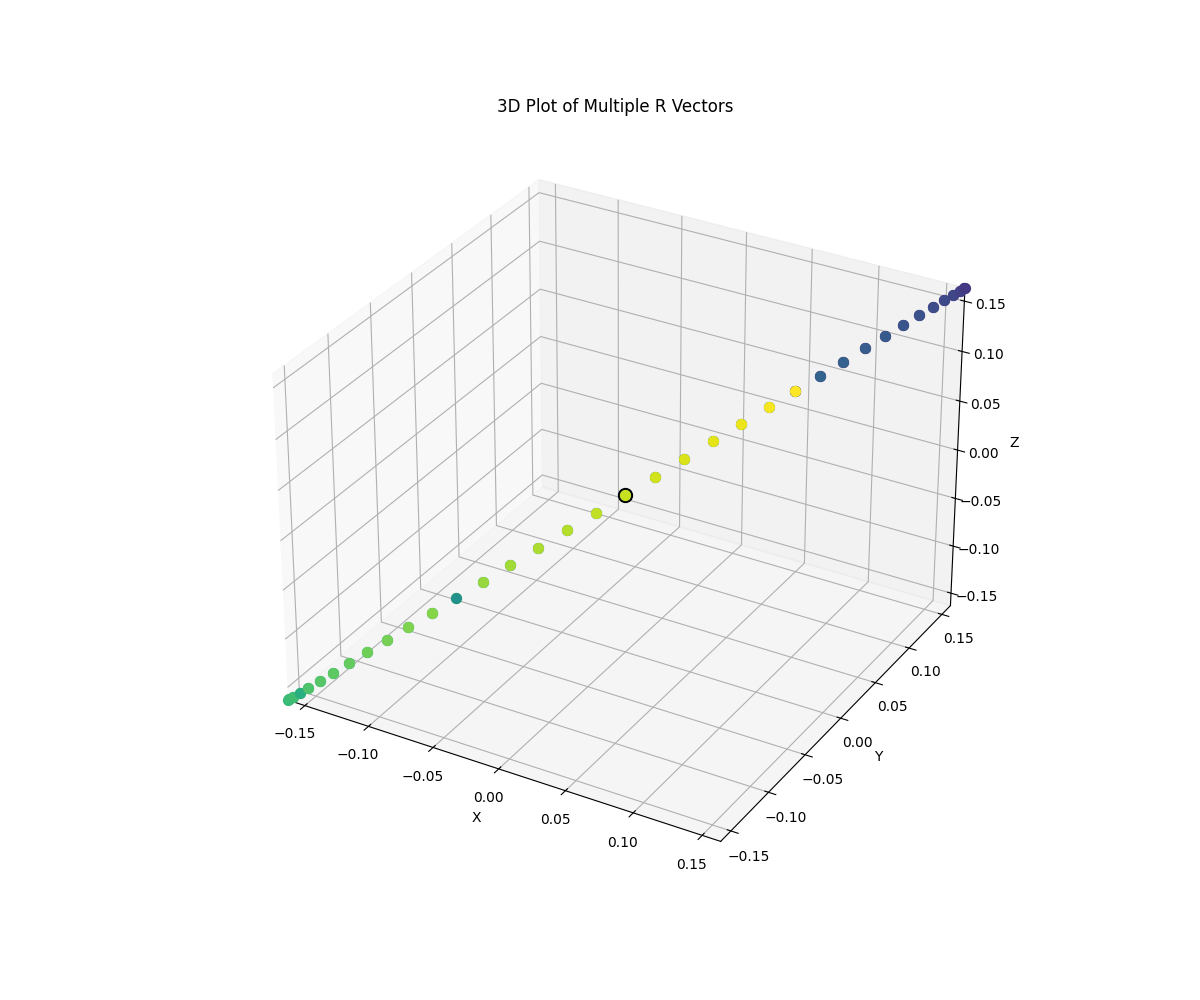
\includegraphics[width=0.8\textwidth]{figures/circle_3d.png}
    \caption{3D visualization of the orthogonal vector configuration}
    \label{fig:example_default_3d}
\end{figure}

\subsubsection{2D Projections}

\begin{figure}[H]
    \centering
    \includegraphics[width=0.45\textwidth]{figures/circle_xy.png}
    \includegraphics[width=0.45\textwidth]{figures/circle_xz.png}
    \includegraphics[width=0.45\textwidth]{figures/circle_yz.png}
    \includegraphics[width=0.45\textwidth]{figures/circle_r0.png}
    \caption{2D projections of the orthogonal vector configuration}
    \label{fig:example_default_2d}
\end{figure}

\subsection{Multiple Vector Generation}

The system supports generating multiple vectors by specifying ranges for the distance and angle parameters. This is particularly useful for exploring the effects of varying parameters on the resulting vectors and for generating complex patterns.

\subsubsection{Distance Range Example}

This example generates multiple vectors with varying distance values (from 1 to 3 in 5 steps) and a fixed angle ($\pi/4$):

\begin{lstlisting}[language=bash]
python generalized/main.py -R 0 0 0 --d-range 1 5 3 -a 0.7854
\end{lstlisting}

\subsubsection{Angle Range Example}

This example generates multiple vectors with a fixed distance (1.5) and varying angle values (from 0 to $\pi$ in 10 steps):

\begin{lstlisting}[language=bash]
python generalized/main.py -R 0 0 0 -d 1.5 --theta-range 0 10 3.14159
\end{lstlisting}

\subsection{Circle Examples}

The system includes three example scripts demonstrating different approaches to generating and visualizing circle and sphere-like patterns. Each example generates 73 points (from 0\textdegree\ to 360\textdegree\ in 5\textdegree\ increments) and plots only the endpoints of the vectors.

\subsubsection{Orthogonal Vector Circle}

The \texttt{example\_circle.py} script generates points using orthogonal vector formulas, creating a sphere-like pattern:

\begin{lstlisting}[language=bash]
python generalized/example_circle.py
\end{lstlisting}

\begin{figure}[H]
    \centering
    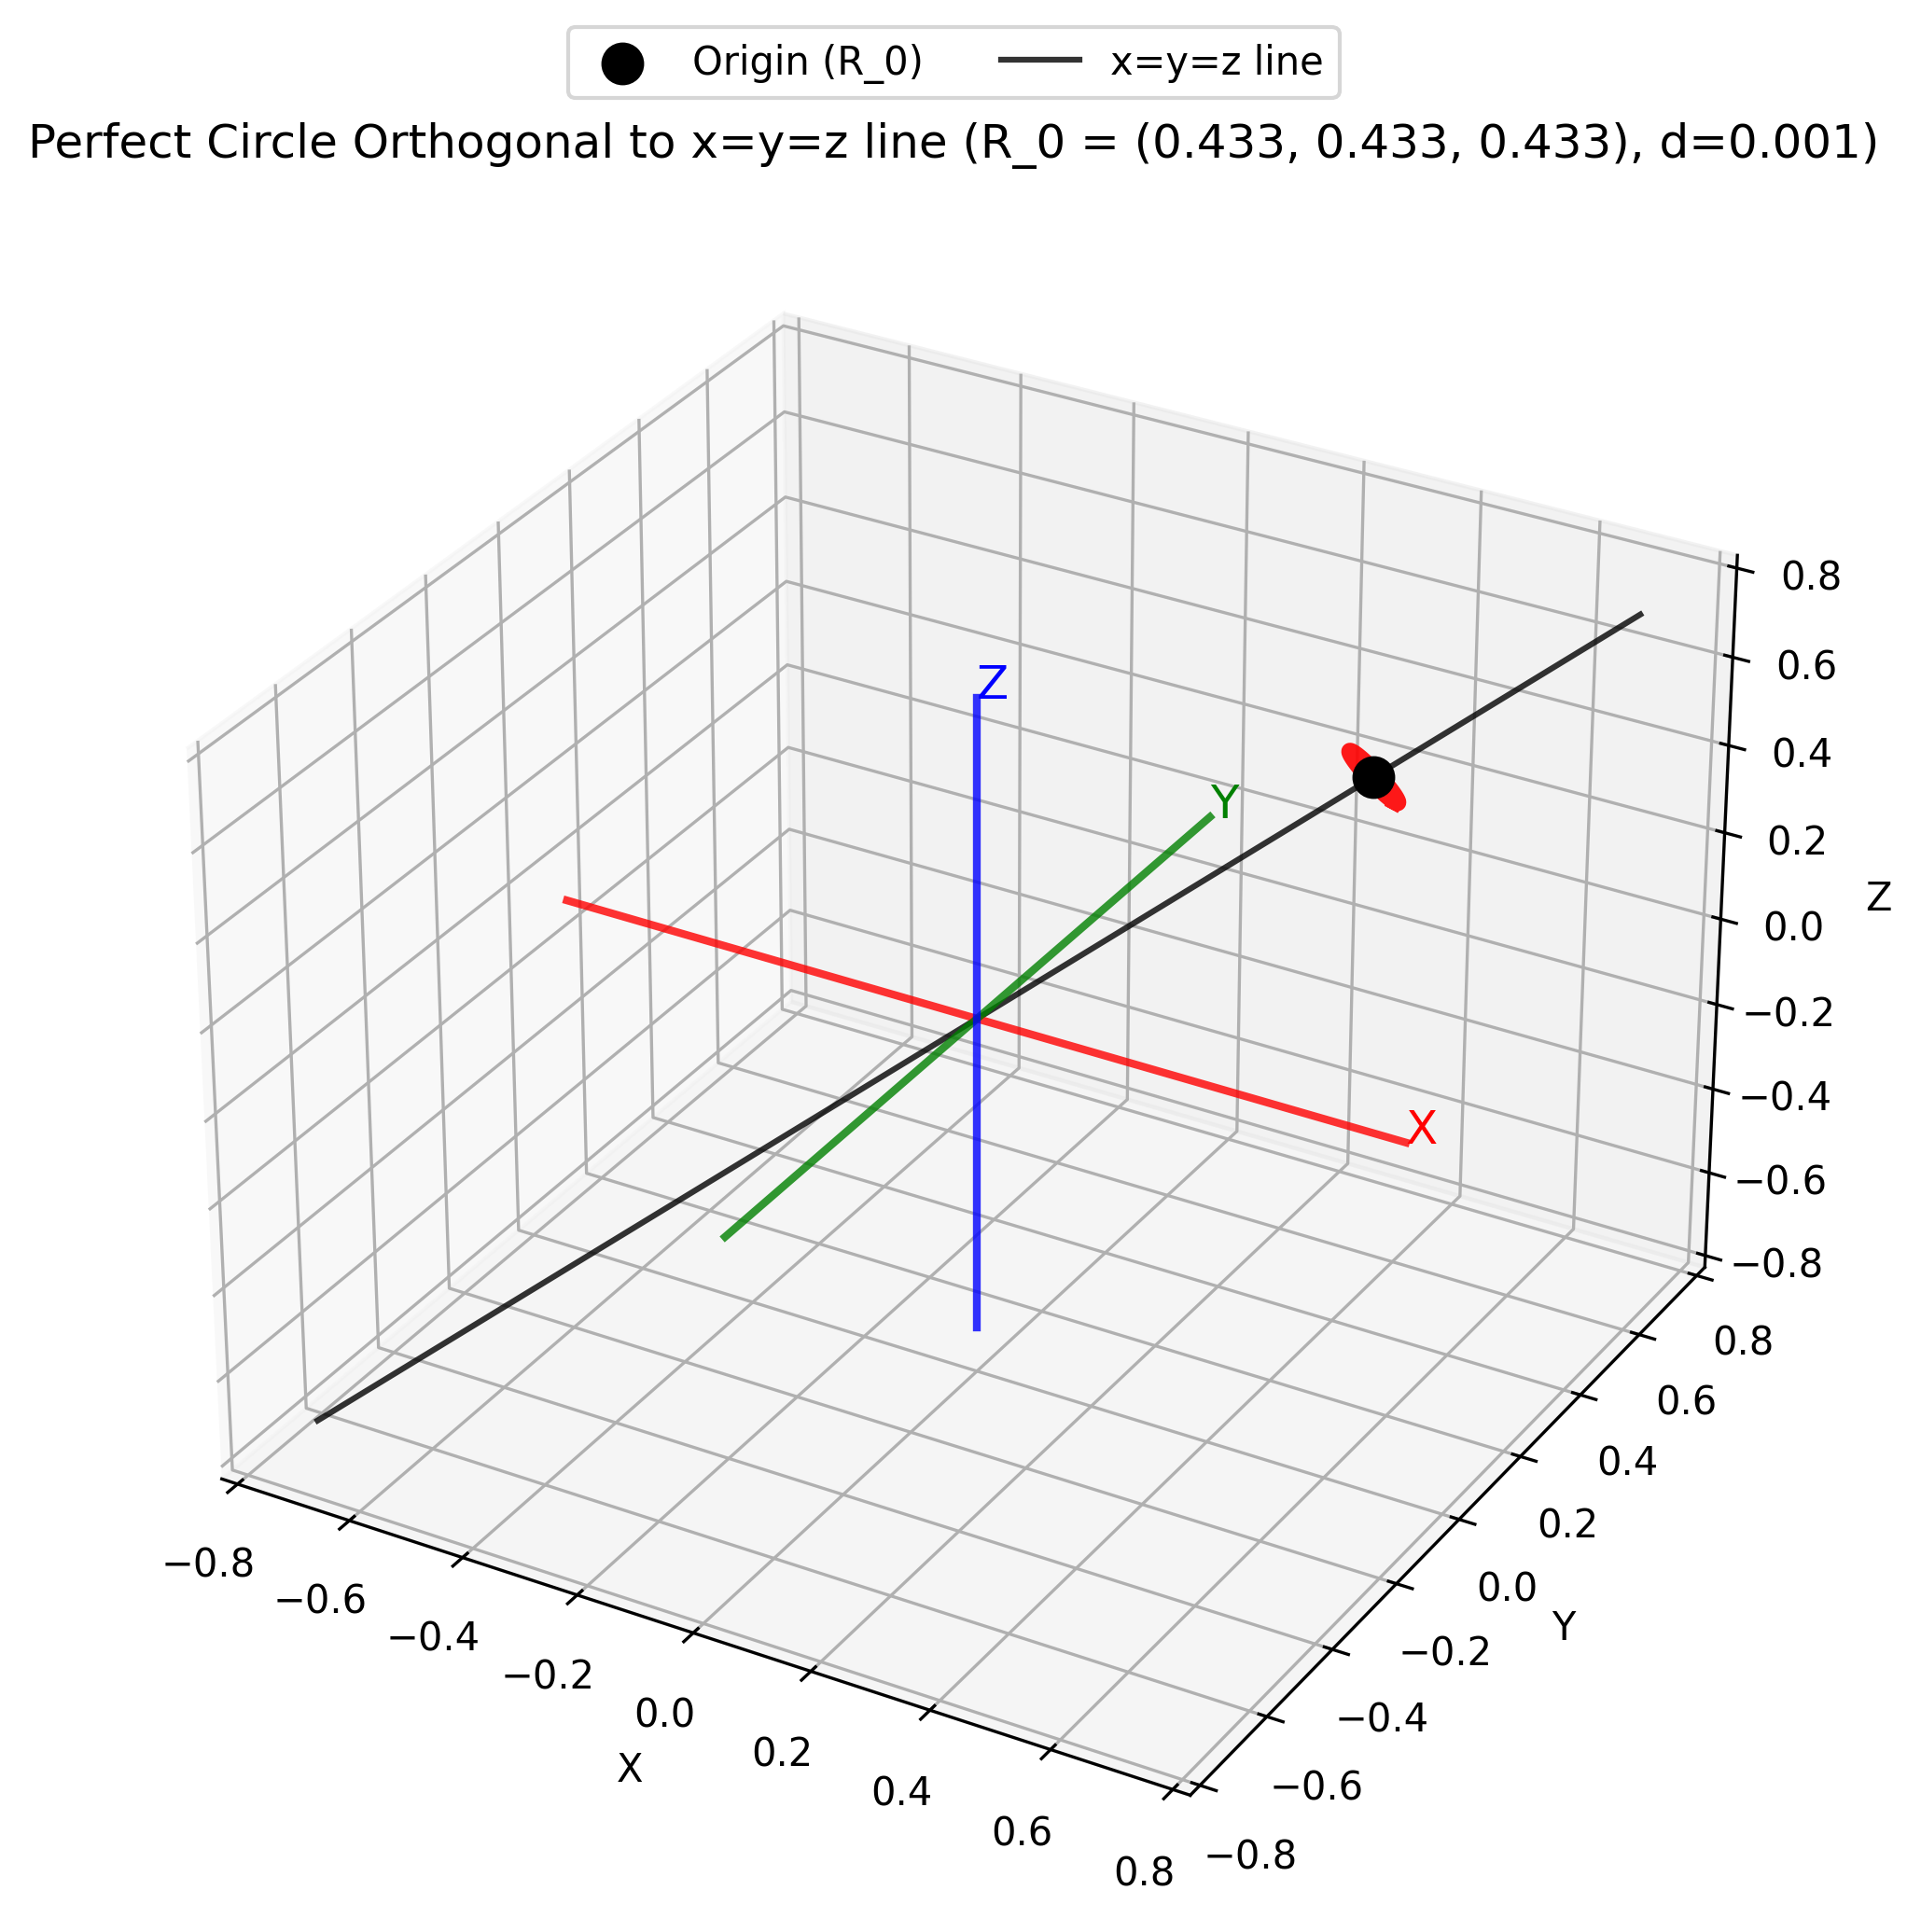
\includegraphics[width=0.8\textwidth]{../../../circle_plots/circle_3d.png}
    \caption{3D visualization of the orthogonal vector circle}
    \label{fig:example_circle_3d}
\end{figure}

\begin{figure}[H]
    \centering
    \begin{minipage}{0.48\textwidth}
        \centering
        \includegraphics[width=\textwidth]{../../../circle_plots/circle_xy.png}
        \caption{XY projection of the orthogonal vector circle}
        \label{fig:example_circle_xy}
    \end{minipage}\hfill
    \begin{minipage}{0.48\textwidth}
        \centering
        \includegraphics[width=\textwidth]{../../../circle_plots/circle_xz.png}
        \caption{XZ projection of the orthogonal vector circle}
        \label{fig:example_circle_xz}
    \end{minipage}
\end{figure}

\begin{figure}[H]
    \centering
    \begin{minipage}{0.48\textwidth}
        \centering
        \includegraphics[width=\textwidth]{../../../circle_plots/circle_yz.png}
        \caption{YZ projection of the orthogonal vector circle}
        \label{fig:example_circle_yz}
    \end{minipage}\hfill
    \begin{minipage}{0.48\textwidth}
        \centering
        \includegraphics[width=\textwidth]{../../../circle_plots/circle_r0.png}
        \caption{Origin plane projection of the orthogonal vector circle}
        \label{fig:example_circle_origin}
    \end{minipage}
\end{figure}

\subsubsection{Traditional XY Circle}

The \texttt{example\_circle\_xy.py} script creates a traditional circle in the XY plane:

\begin{lstlisting}[language=bash]
python generalized/example_circle_xy.py
\end{lstlisting}

\begin{figure}[H]
    \centering
    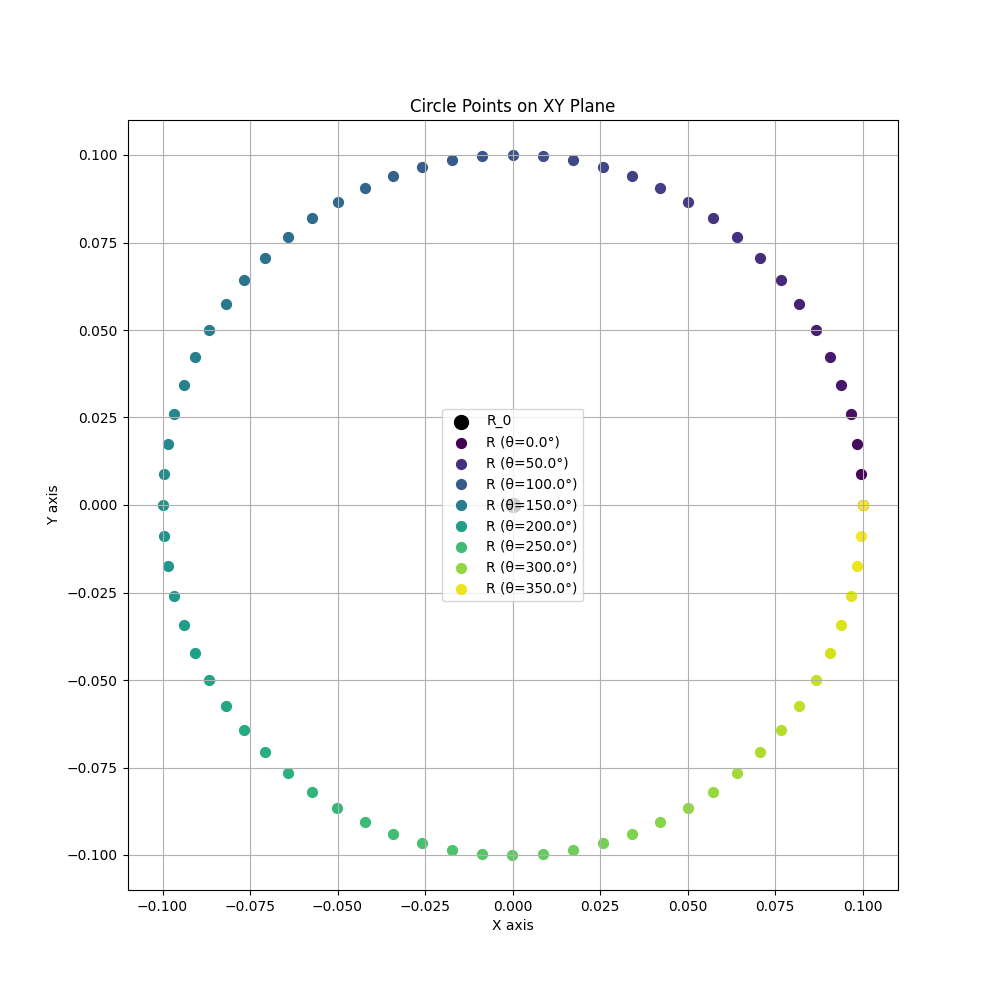
\includegraphics[width=0.8\textwidth]{figures/xy_circle.png}
    \caption{Traditional circle in the XY plane}
    \label{fig:example_xy_circle}
\end{figure}

\begin{figure}[H]
    \centering
    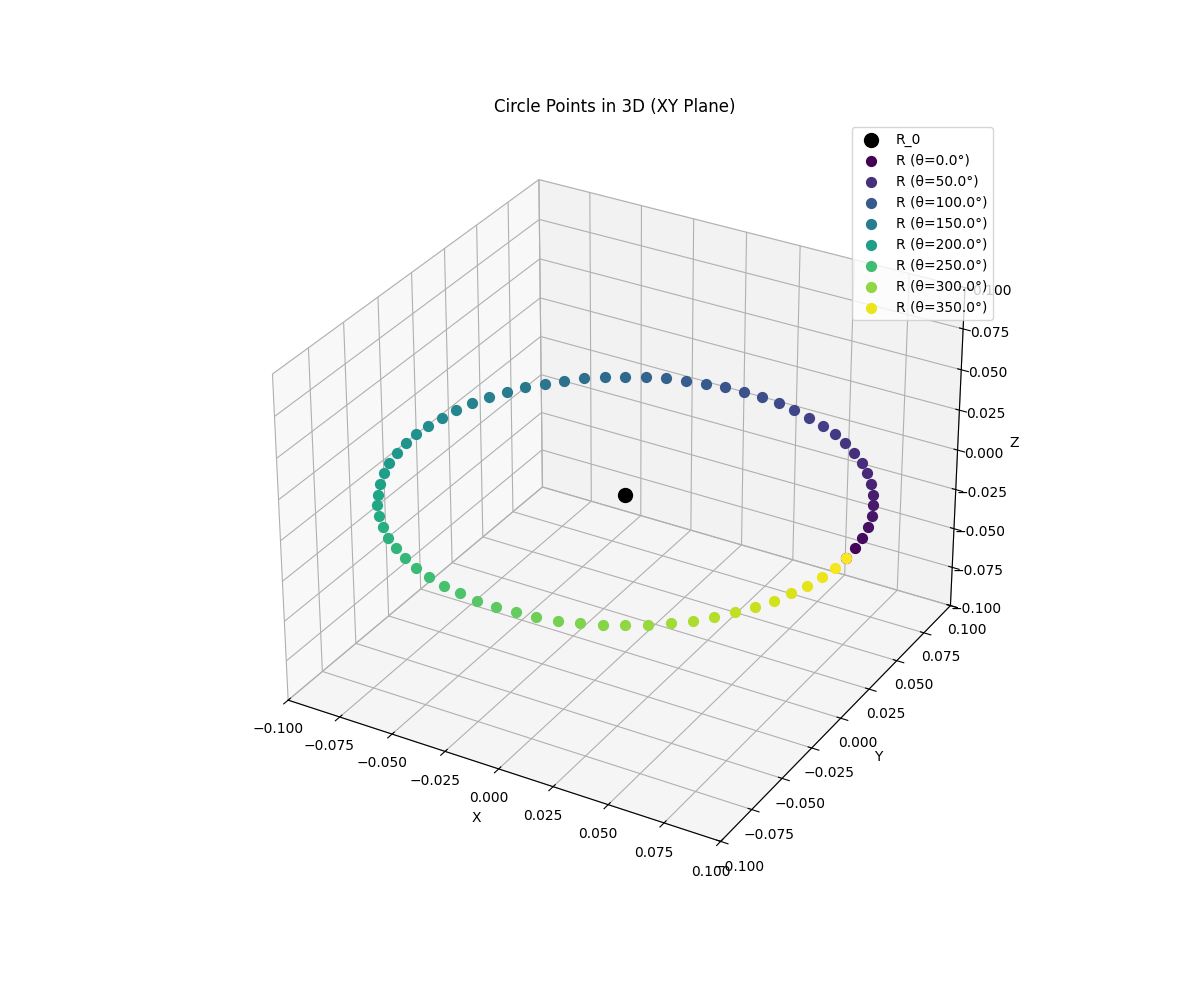
\includegraphics[width=0.8\textwidth]{../../../circle_plots/3d_xy_circle.png}
    \caption{3D visualization of the traditional XY circle}
    \label{fig:example_3d_xy_circle}
\end{figure}

\subsubsection{Improved Orthogonal Vector Circle}

The \texttt{example\_orthogonal\_circle.py} script is similar to the first example but with improved visualization:

\begin{lstlisting}[language=bash]
python generalized/example_orthogonal_circle.py
\end{lstlisting}

\begin{figure}[H]
    \centering
    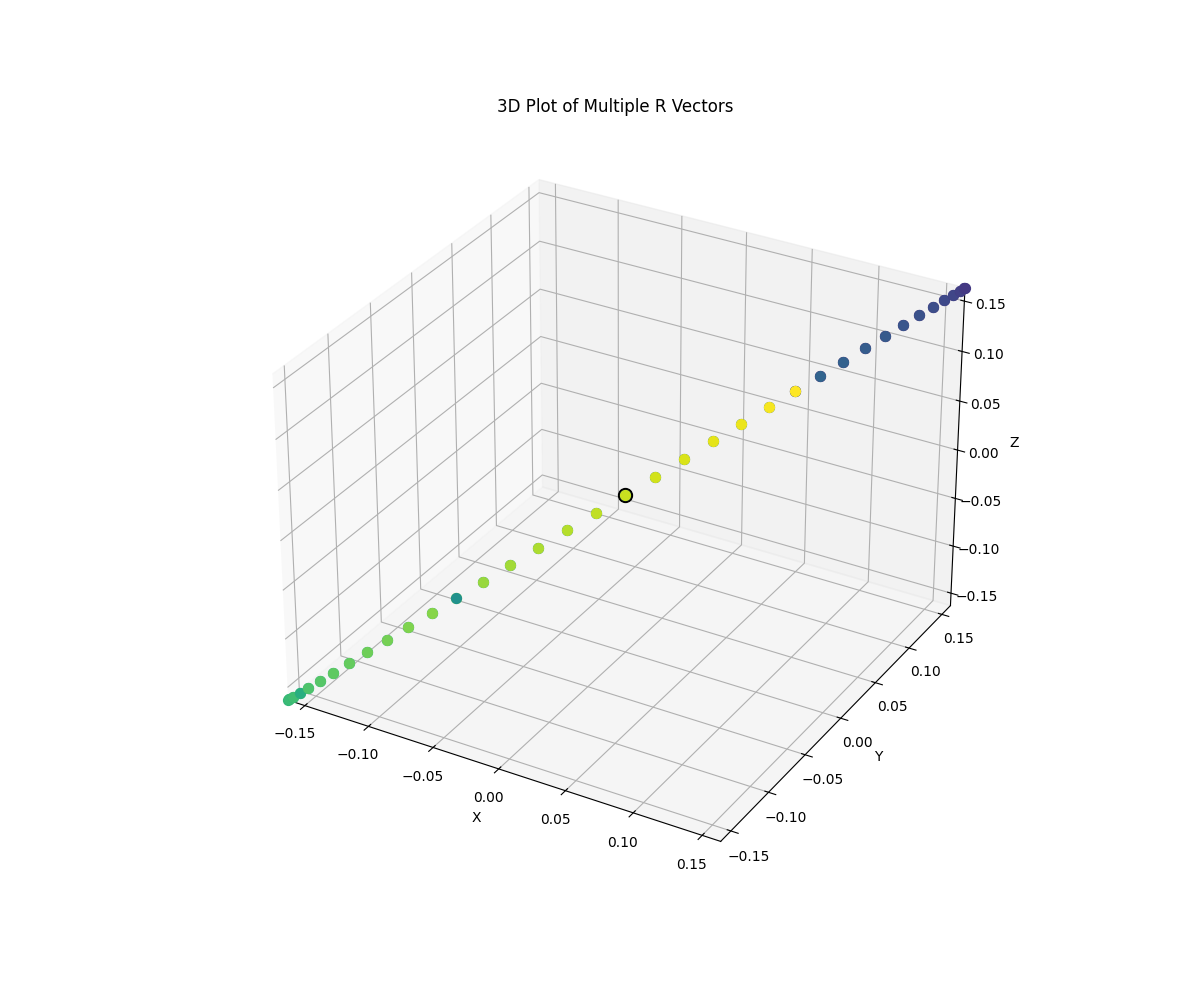
\includegraphics[width=0.8\textwidth]{../../../circle_plots/orthogonal_3d.png}
    \caption{3D visualization of the improved orthogonal vector circle}
    \label{fig:example_orthogonal_3d}
\end{figure}

\begin{figure}[H]
    \centering
    \begin{minipage}{0.48\textwidth}
        \centering
        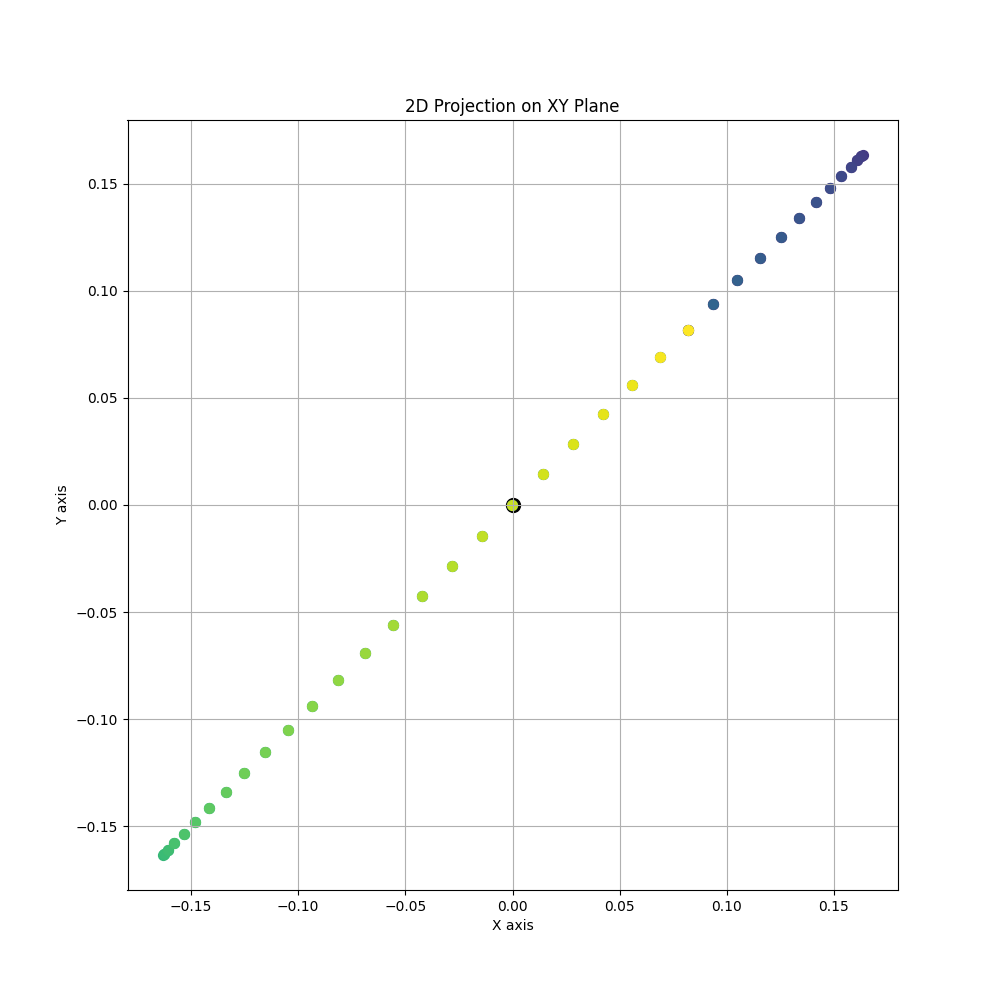
\includegraphics[width=\textwidth]{../../../circle_plots/orthogonal_xy.png}
        \caption{XY projection of the improved orthogonal vector circle}
        \label{fig:example_orthogonal_xy}
    \end{minipage}\hfill
    \begin{minipage}{0.48\textwidth}
        \centering
        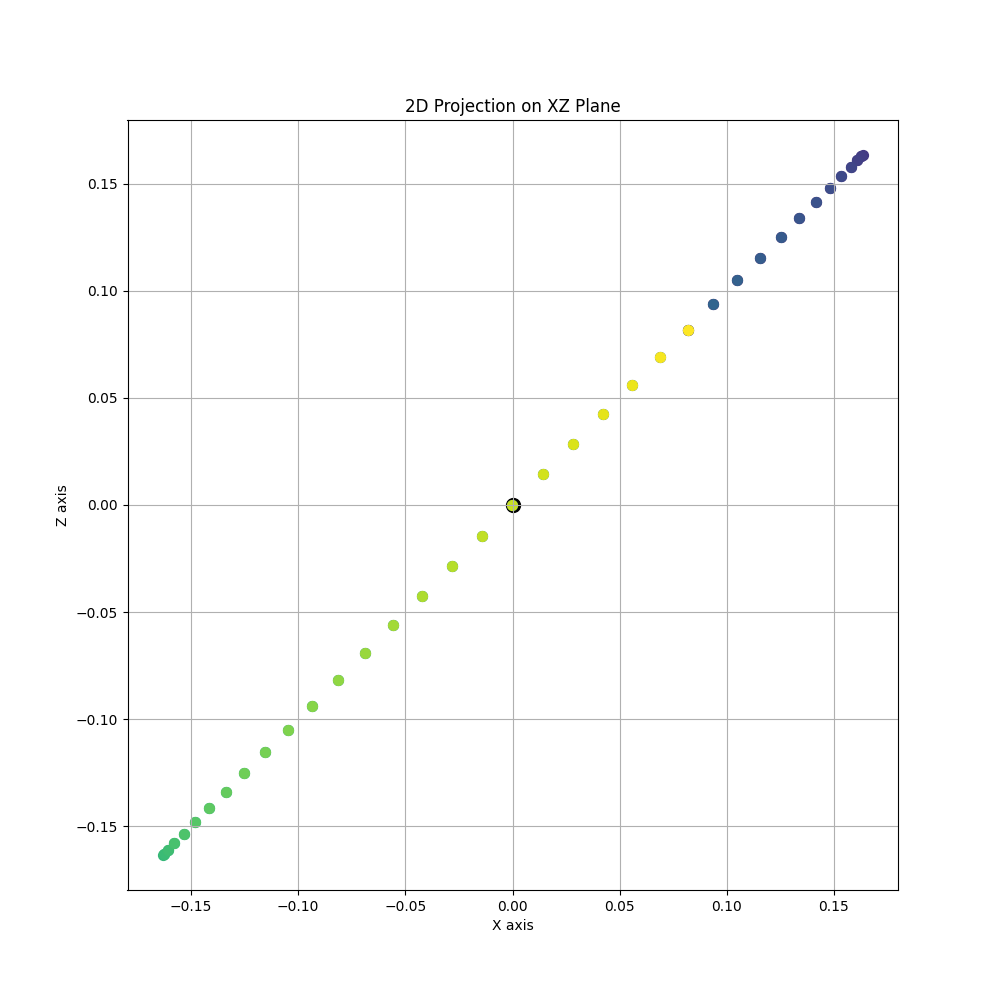
\includegraphics[width=\textwidth]{../../../circle_plots/orthogonal_xz.png}
        \caption{XZ projection of the improved orthogonal vector circle}
        \label{fig:example_orthogonal_xz}
    \end{minipage}
\end{figure}

\begin{figure}[H]
    \centering
    \begin{minipage}{0.48\textwidth}
        \centering
        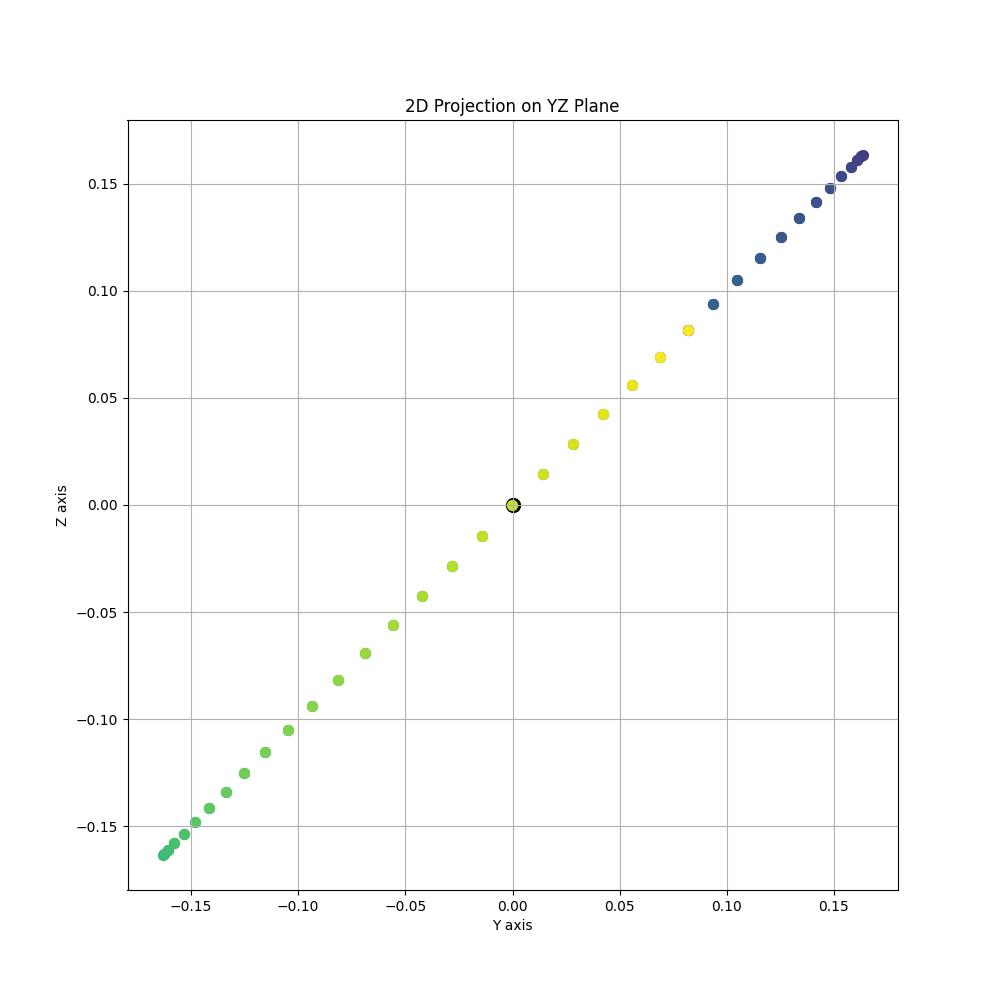
\includegraphics[width=\textwidth]{../../../circle_plots/orthogonal_yz.png}
        \caption{YZ projection of the improved orthogonal vector circle}
        \label{fig:example_orthogonal_yz}
    \end{minipage}\hfill
    \begin{minipage}{0.48\textwidth}
        \centering
        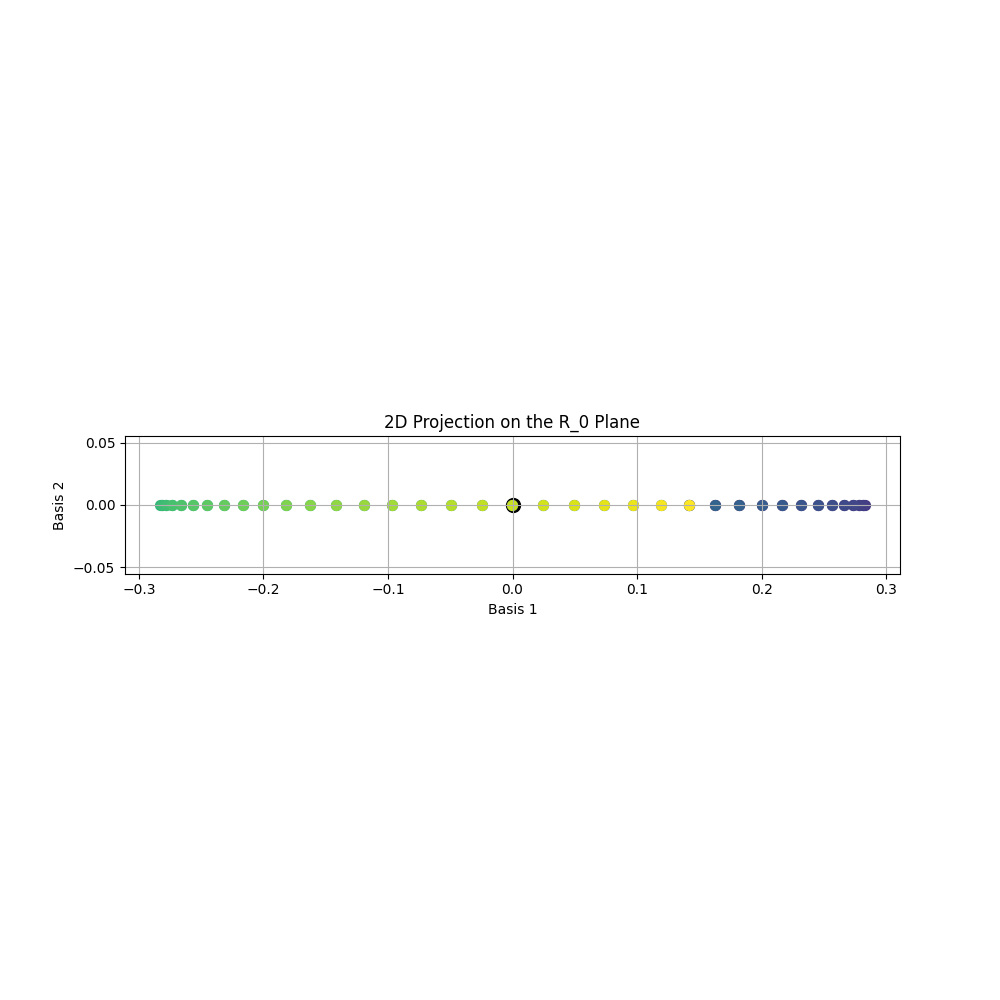
\includegraphics[width=\textwidth]{../../../circle_plots/orthogonal_r0.png}
        \caption{Origin plane projection of the improved orthogonal vector circle}
        \label{fig:example_orthogonal_origin}
    \end{minipage}
\end{figure}








\subsection{Perfect Orthogonal Circle Generation}

This section presents the implementation of a perfect circle generator in the plane orthogonal to the x=y=z line. This implementation ensures that all points on the circle are exactly at the specified distance from the origin and perfectly orthogonal to the (1,1,1) direction.

\subsubsection{Implementation Approach}

The perfect orthogonal circle is generated using normalized basis vectors that span the plane orthogonal to the (1,1,1) direction:

\begin{itemize}
    \item Basis vector 1: $[1, -1/2, -1/2]$ (normalized)
    \item Basis vector 2: $[0, -1/2, 1/2]$ (normalized)
\end{itemize}

Points on the circle are generated using the parametric circle equation with these basis vectors:

\begin{align}
\vec{p} = \vec{R}_0 + d \cdot (\cos(\theta) \cdot \vec{basis}_1 + \sin(\theta) \cdot \vec{basis}_2)
\end{align}

where $\vec{R}_0$ is the origin point, $d$ is the distance parameter, and $\theta$ ranges from 0 to $2\pi$.

\subsubsection{Verification Results}

The implementation was verified with the following parameters:
\begin{itemize}
    \item Origin vector (R\_0): [0, 0, 0]
    \item Distance parameter (d): 1.0
    \item Number of points: 73 (5-degree increments)
\end{itemize}

Verification results confirm perfect circle properties:
\begin{itemize}
    \item Mean distance from origin: exactly 1.0
    \item Standard deviation of distances: 8.01e-17 (effectively 0)
    \item Min/max distance ratio: 1.0000000000000004 (effectively 1.0)
    \item Maximum dot product with (1,1,1): 1.11e-16 (effectively 0)
    \item Average dot product with (1,1,1): 2.88e-17 (effectively 0)
\end{itemize}

\begin{figure}[H]
    \centering
    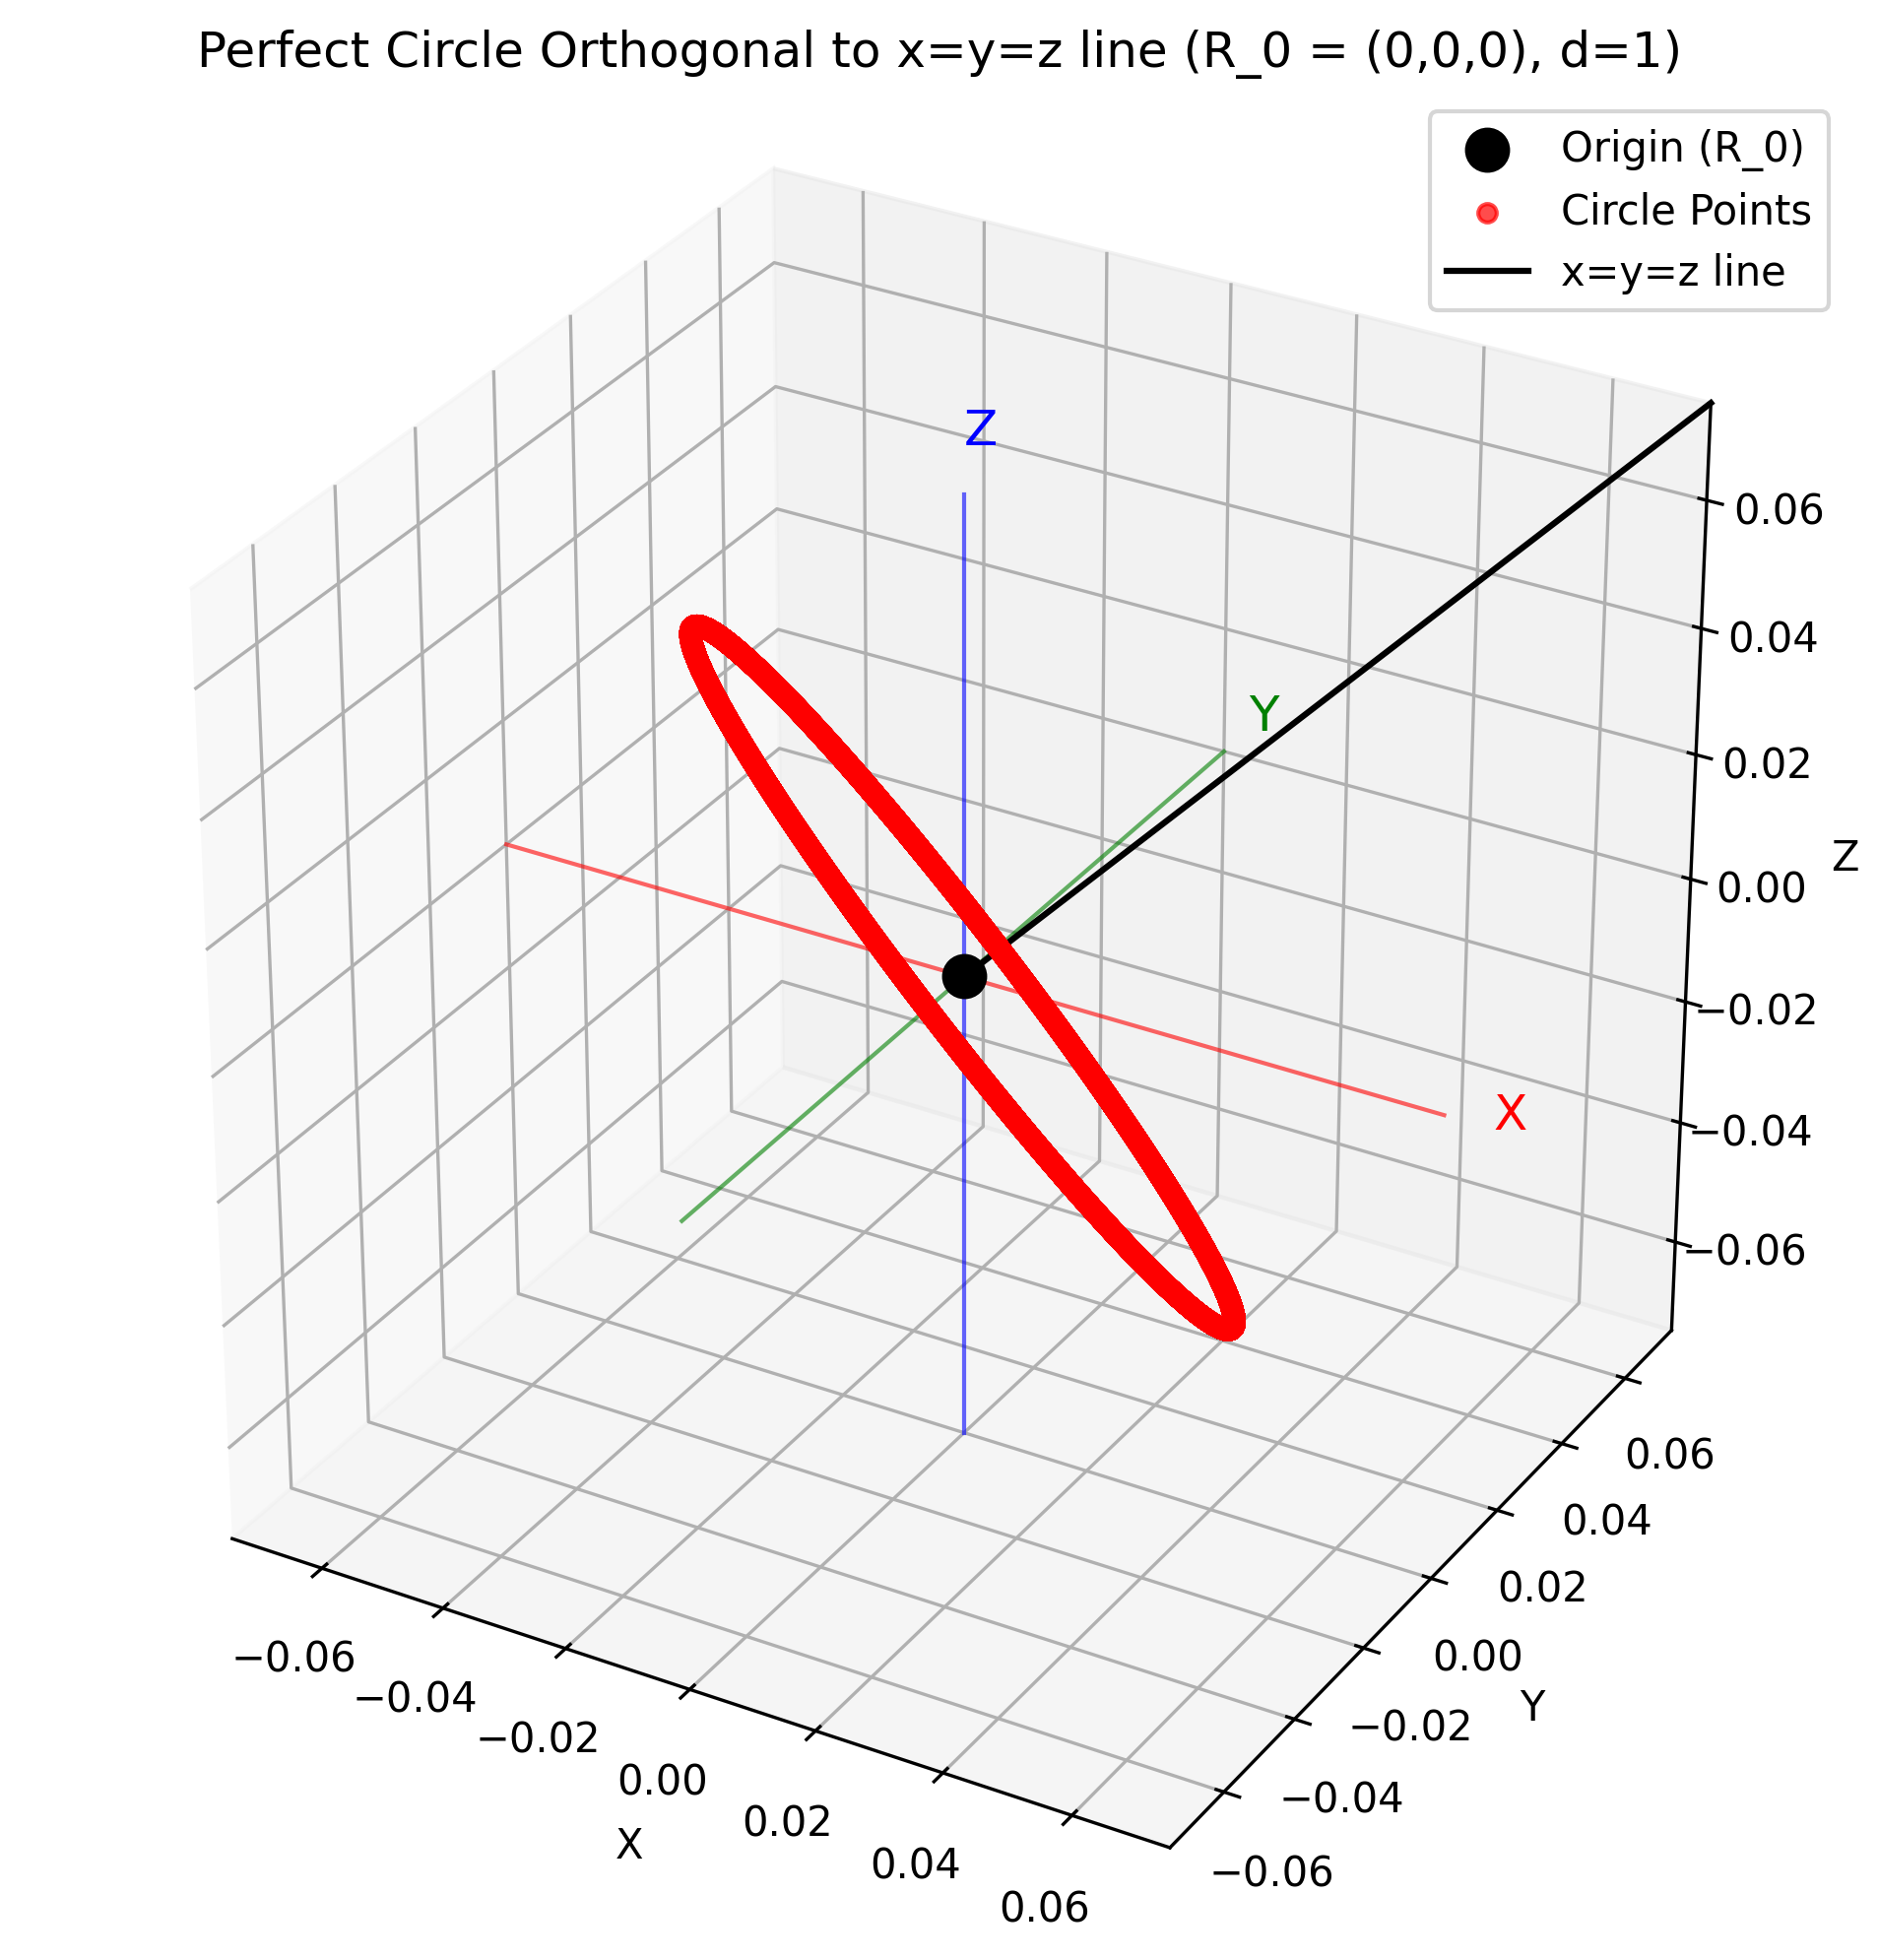
\includegraphics[width=0.8\textwidth]{../../../perfect_circle_output/perfect_circle_3d.png}
    \caption{3D visualization of the perfect circle orthogonal to the x=y=z line}
    \label{fig:perfect_circle_3d}
\end{figure}

\begin{figure}[H]
    \centering
    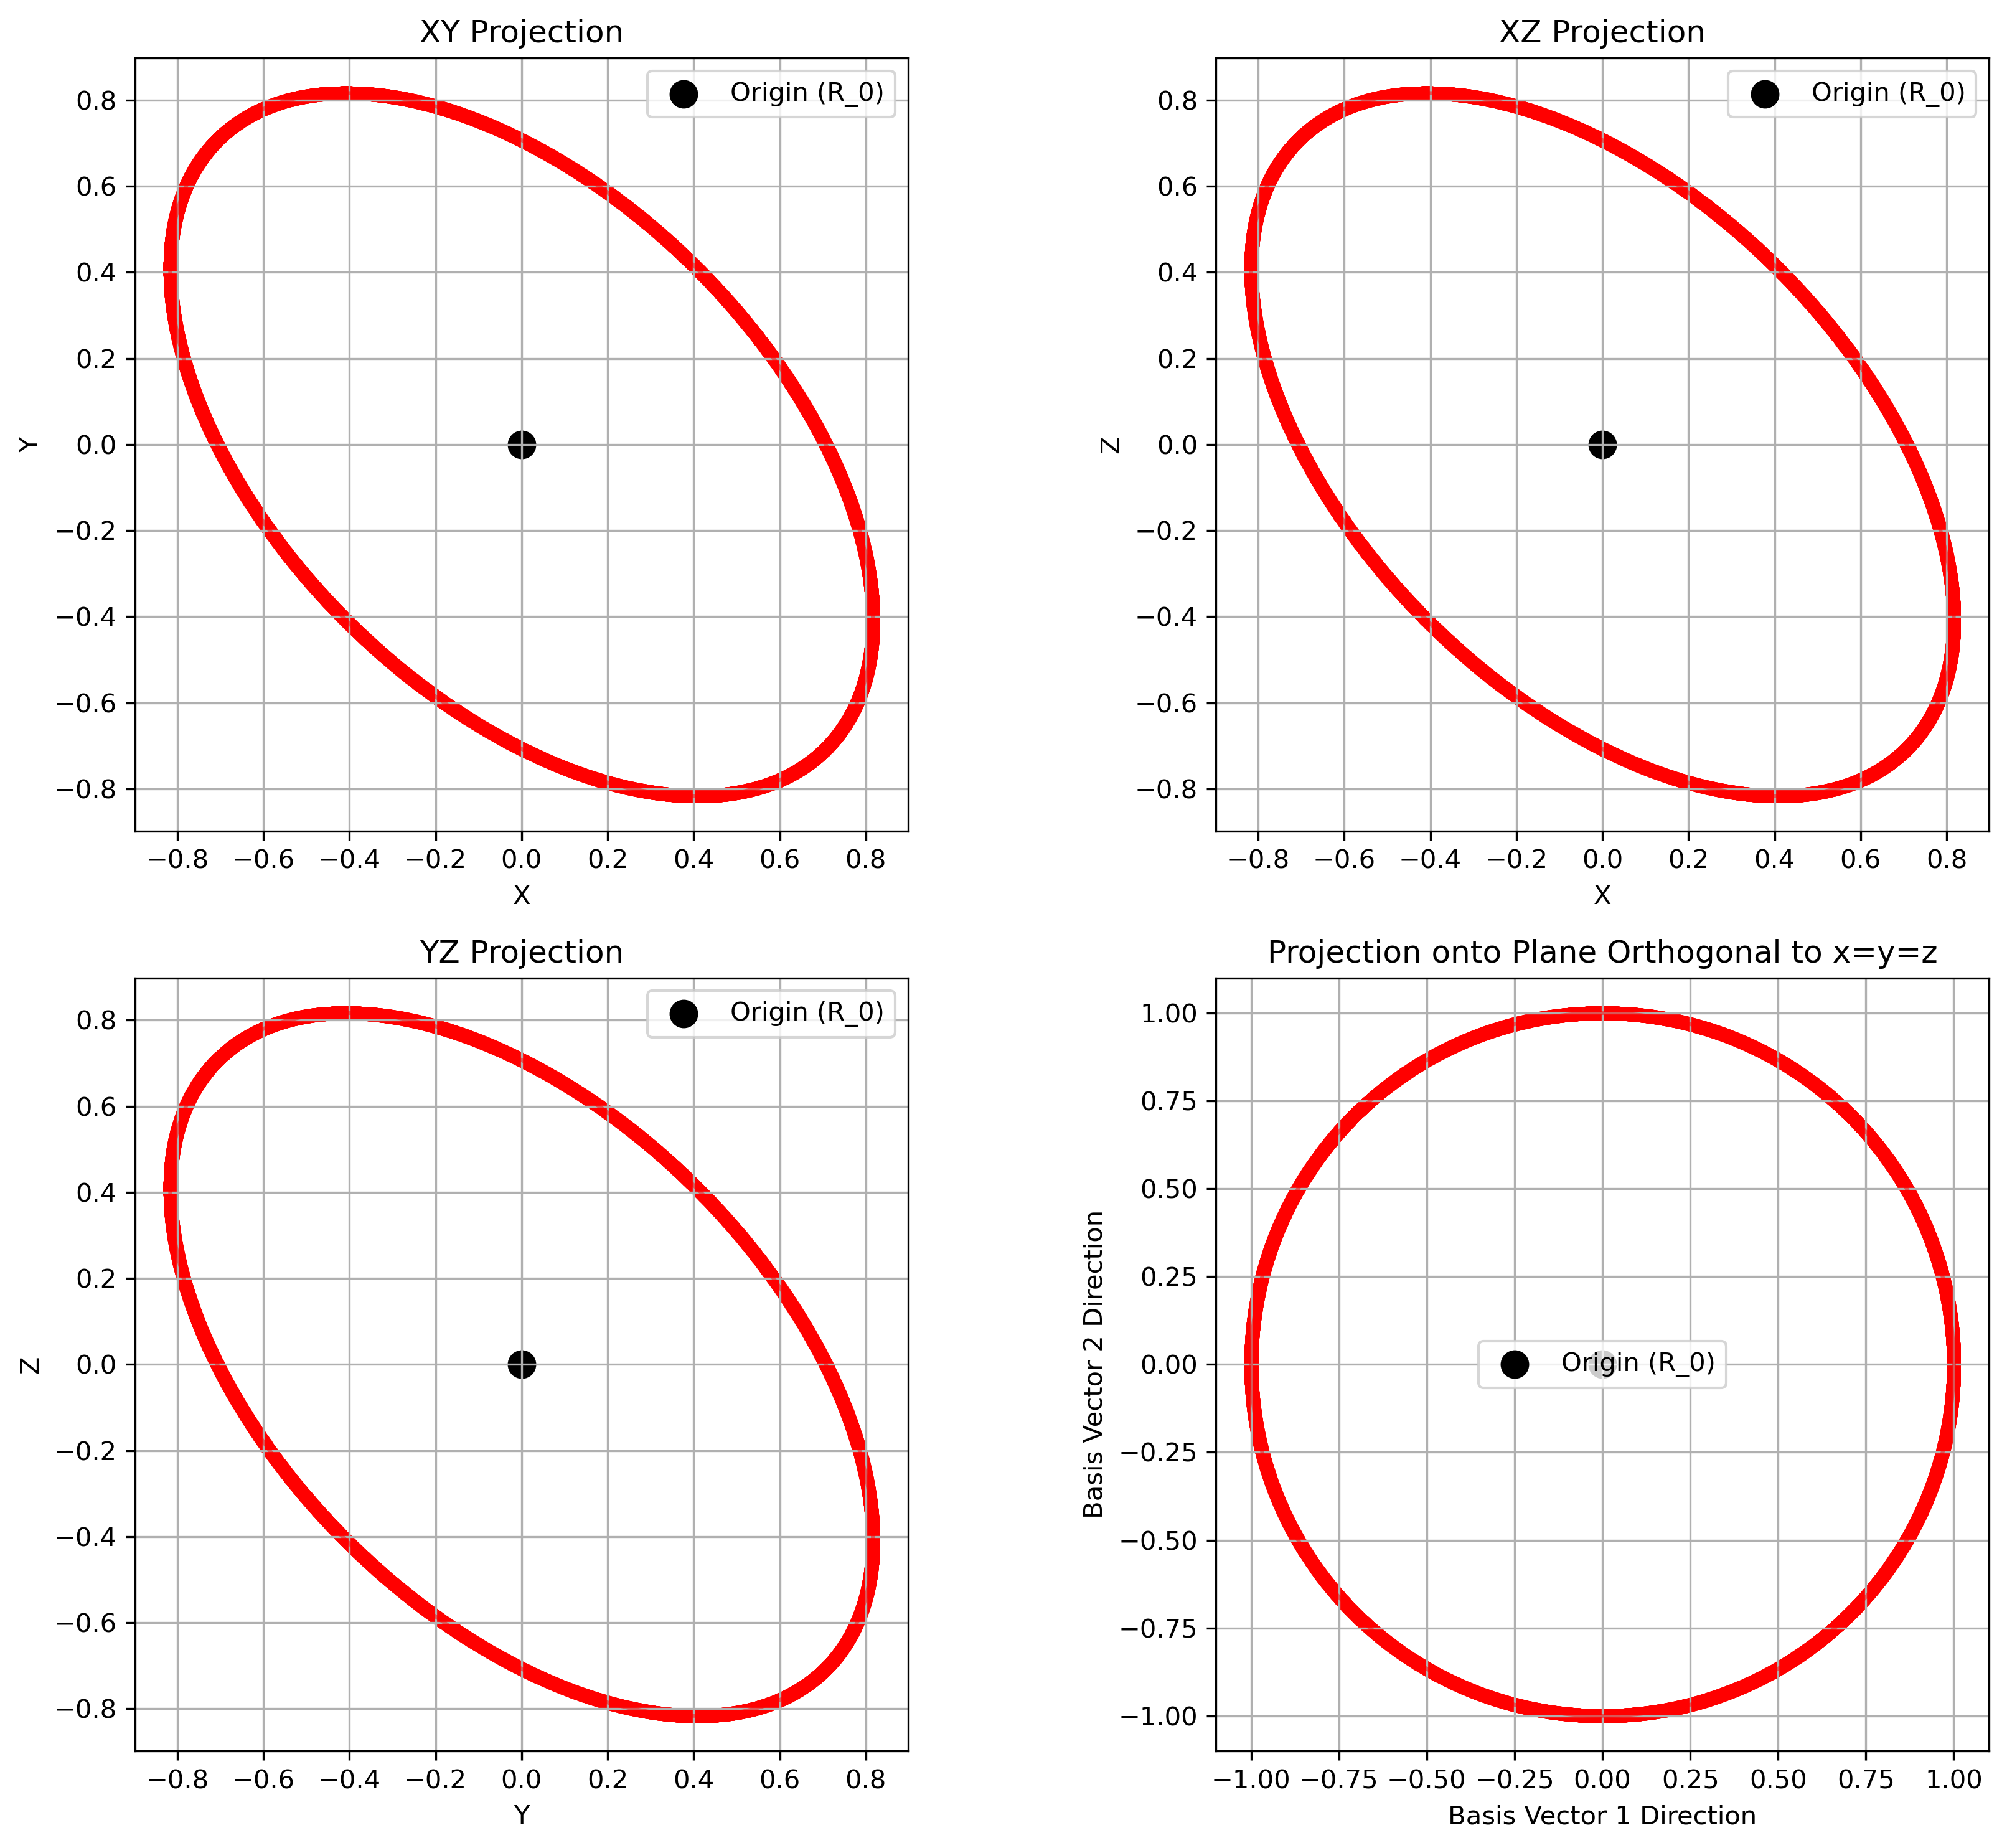
\includegraphics[width=0.8\textwidth]{../../../perfect_circle_output/perfect_circle_projections.png}
    \caption{Projections of the perfect circle onto coordinate planes and orthogonal plane}
    \label{fig:perfect_circle_projections}
\end{figure}

\begin{figure}[H]
    \centering
    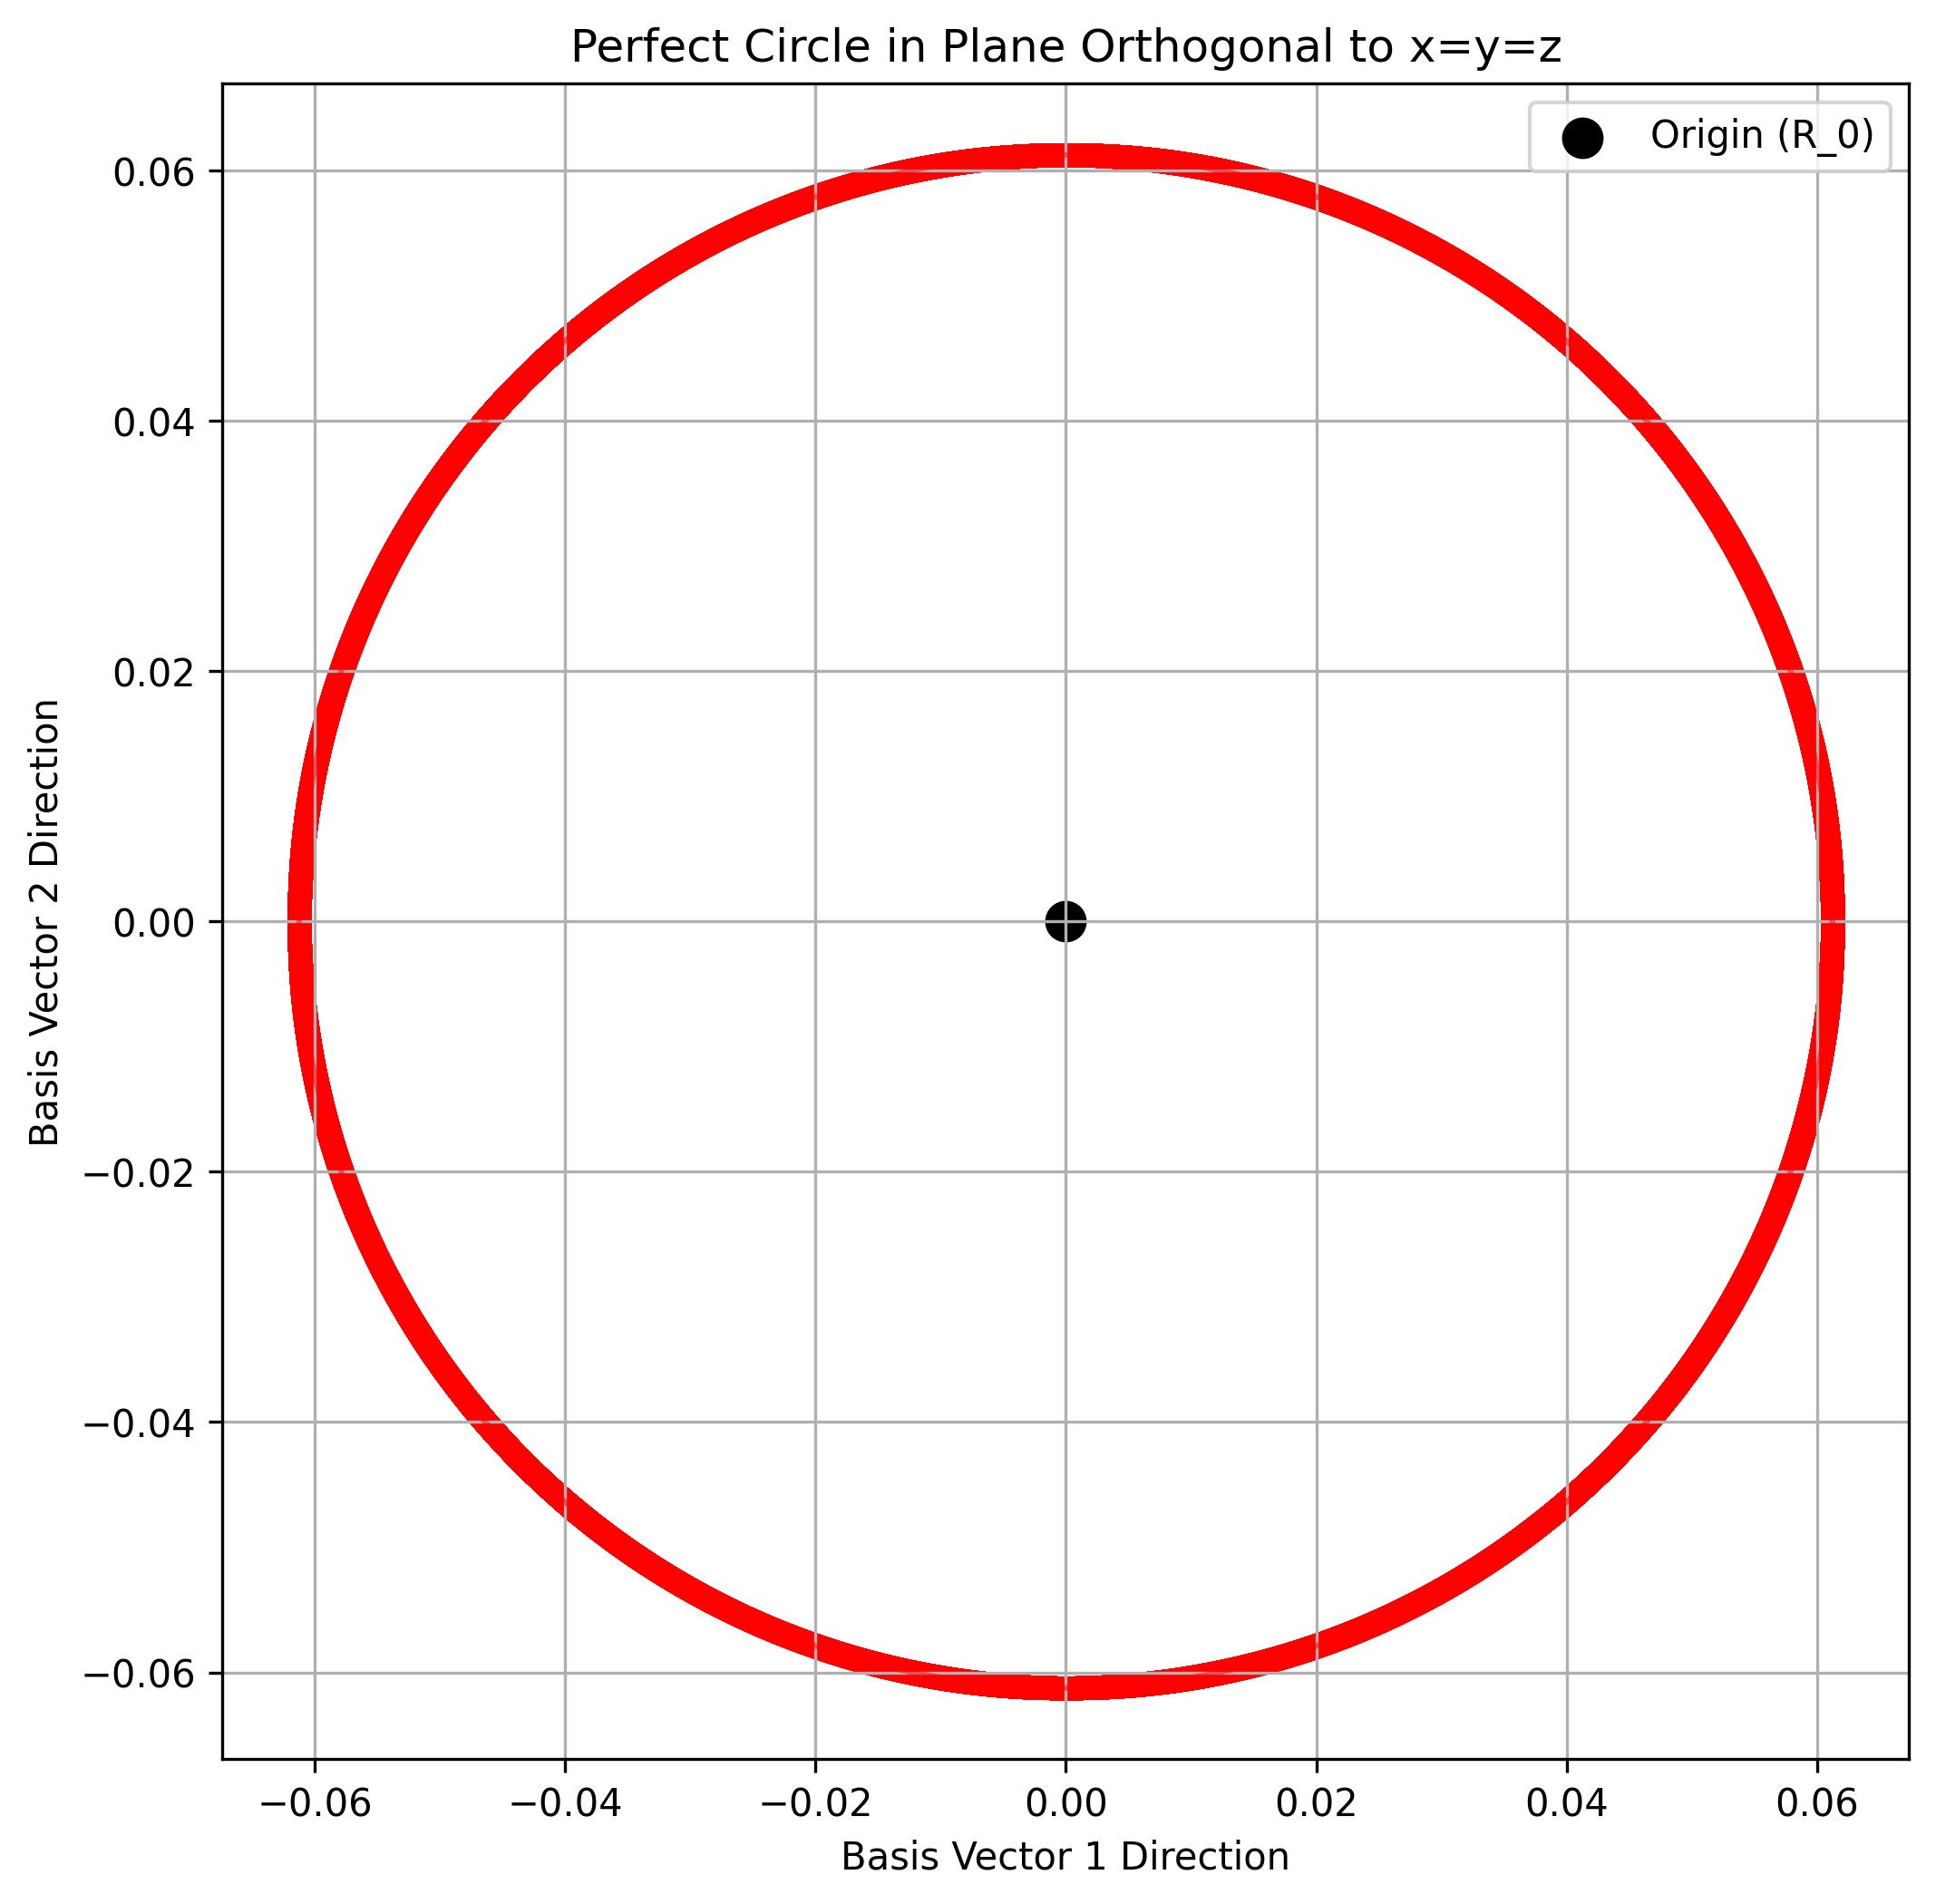
\includegraphics[width=0.8\textwidth]{../../../perfect_circle_output/perfect_circle_orthogonal_plane.png}
    \caption{Perfect circle projected onto the plane orthogonal to the x=y=z line}
    \label{fig:perfect_circle_orthogonal}
\end{figure}

\subsection{Orthogonality Test Results}

This section presents the results of comprehensive tests verifying the orthogonality of generated vectors to the x=y=z line. These tests confirm that the implementation using basis vectors correctly ensures orthogonality to the (1,1,1) direction.

\subsubsection{Single Vector Orthogonality Test}

A test was conducted with the following parameters:
\begin{itemize}
    \item Origin vector (R\_0): [1, 1, 1]
    \item Distance parameter (d): 2.0
    \item Angle parameter ($\theta$): $\pi/4$ (45 degrees)
\end{itemize}

The test verified that the displacement vector (R - R\_0) is orthogonal to the (1,1,1) direction by calculating the dot product, which was effectively zero (within floating-point precision).

\begin{figure}[H]
    \centering
    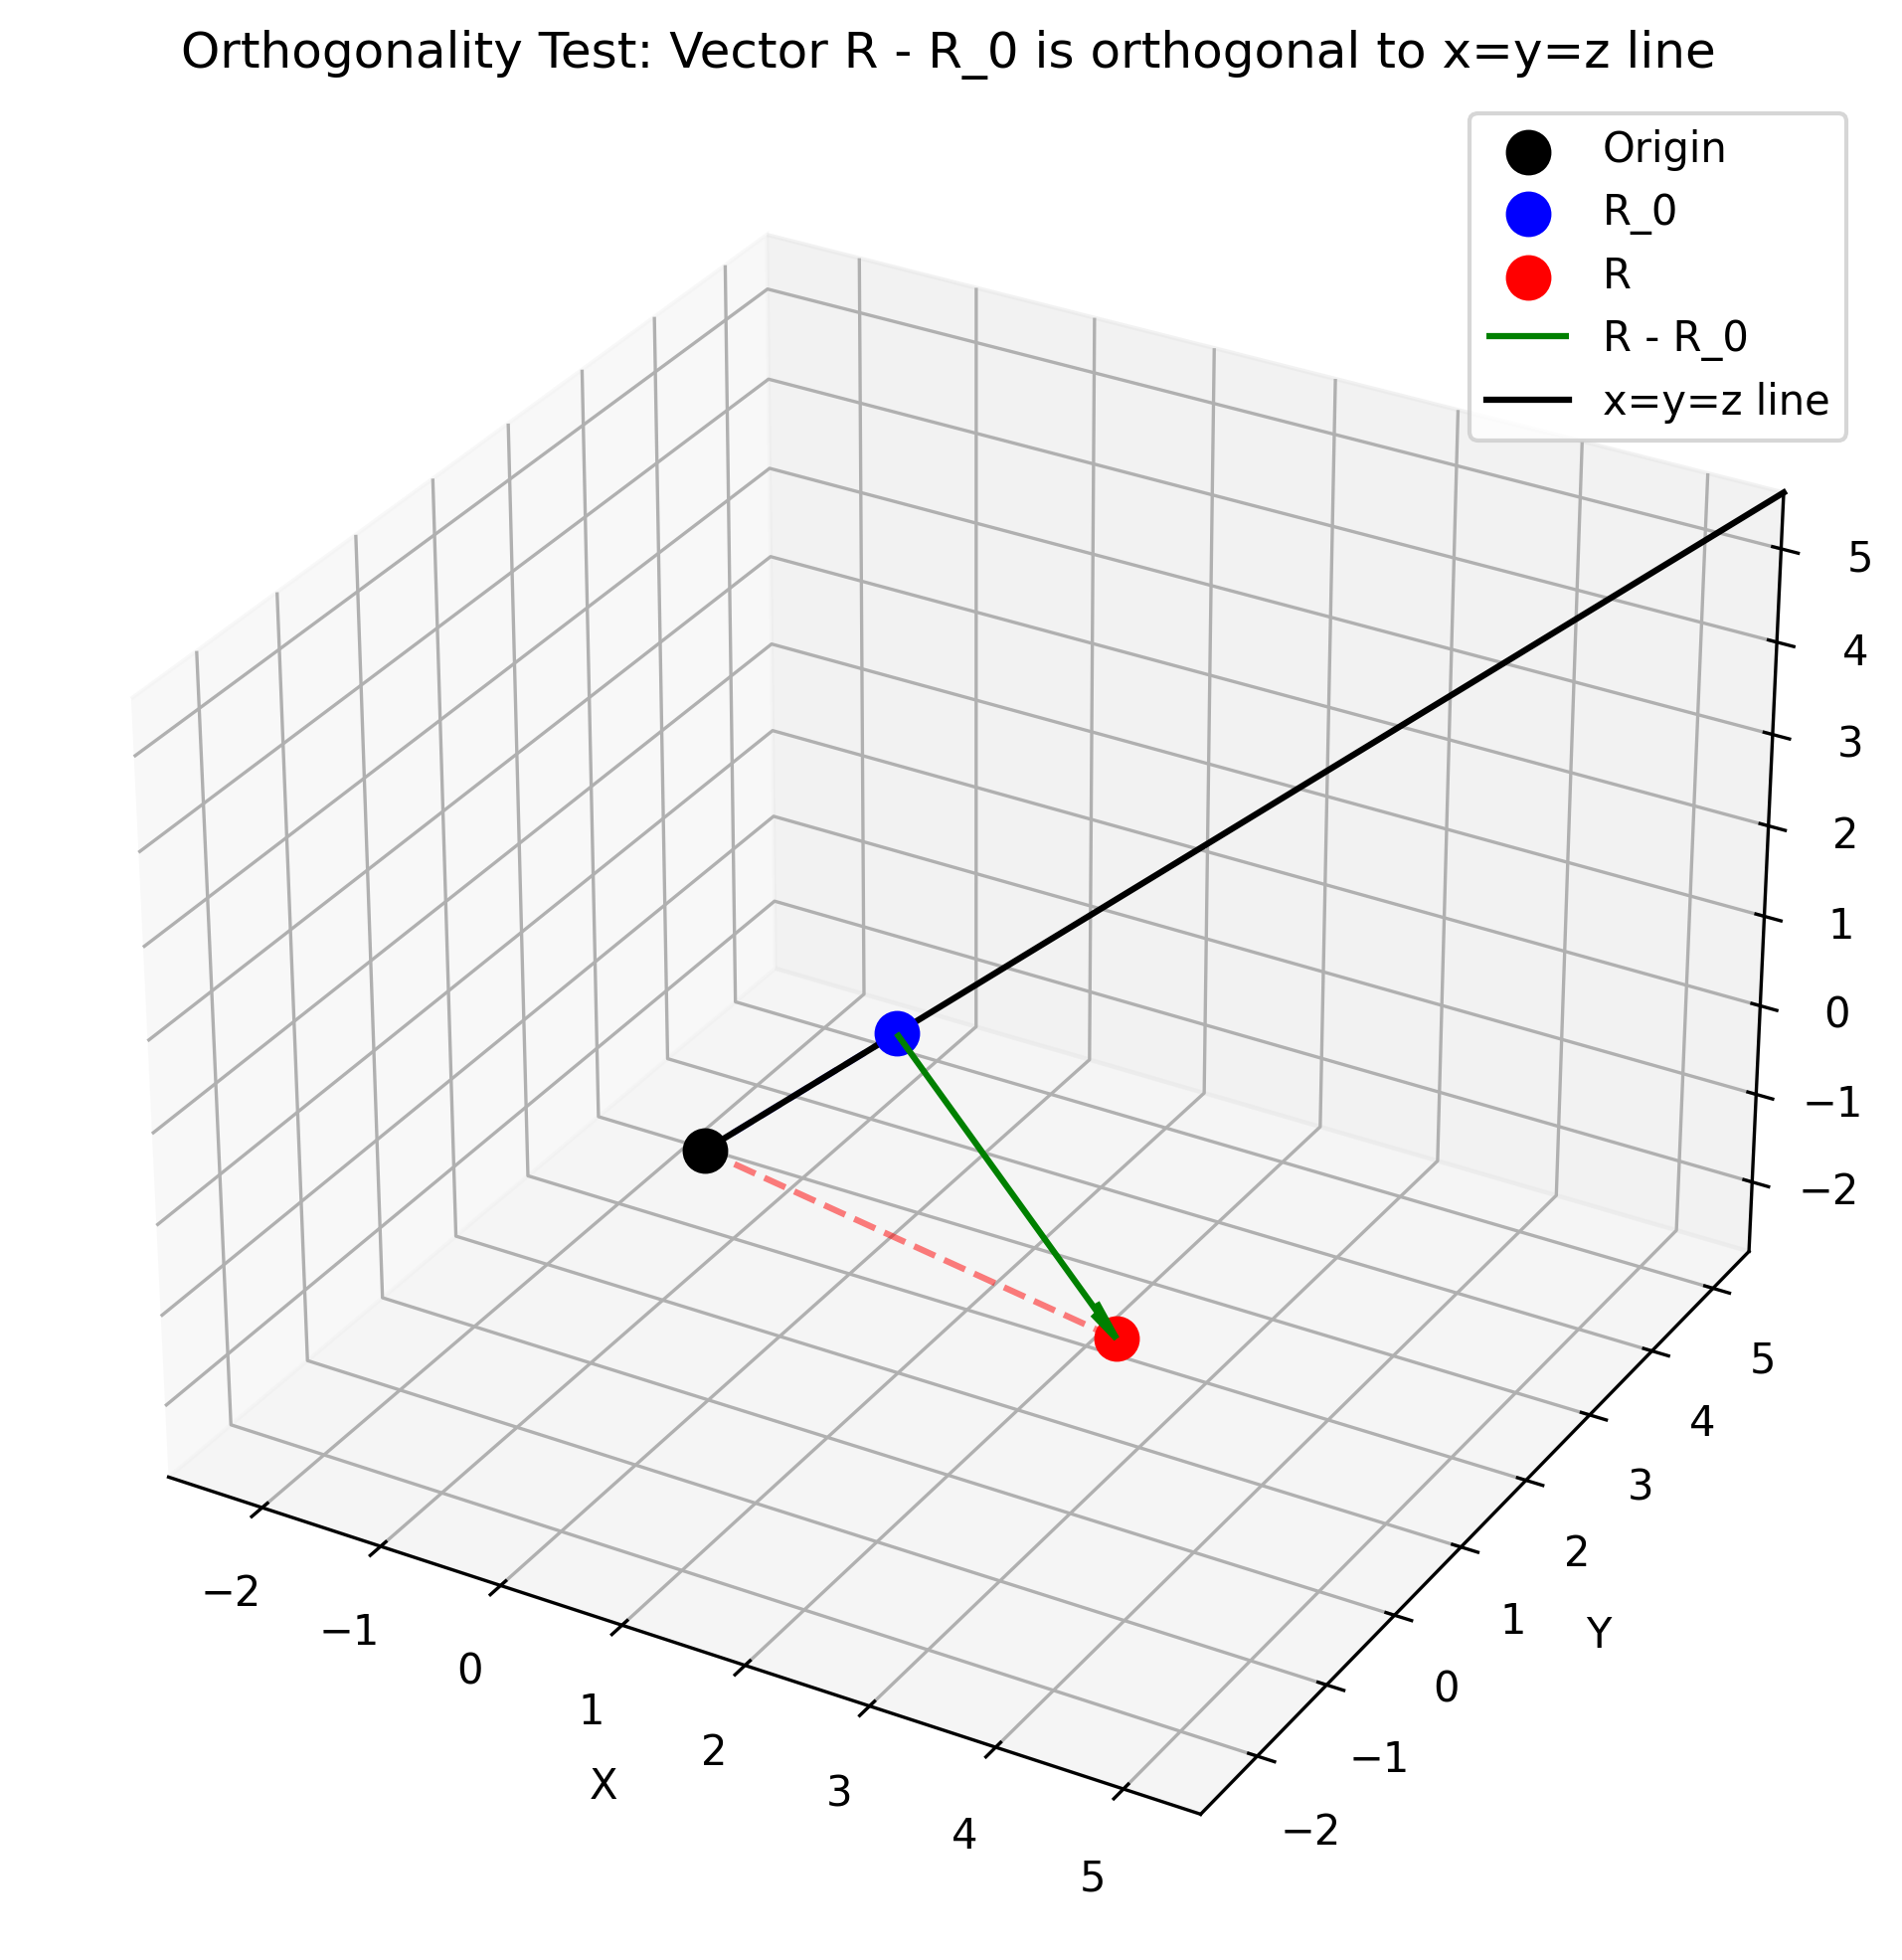
\includegraphics[width=0.8\textwidth]{figures/orthogonality_test/orthogonality_test_3d.png}
    \caption{3D visualization showing the orthogonality of the displacement vector to the x=y=z line}
    \label{fig:orthogonality_test_3d}
\end{figure}

\begin{figure}[H]
    \centering
    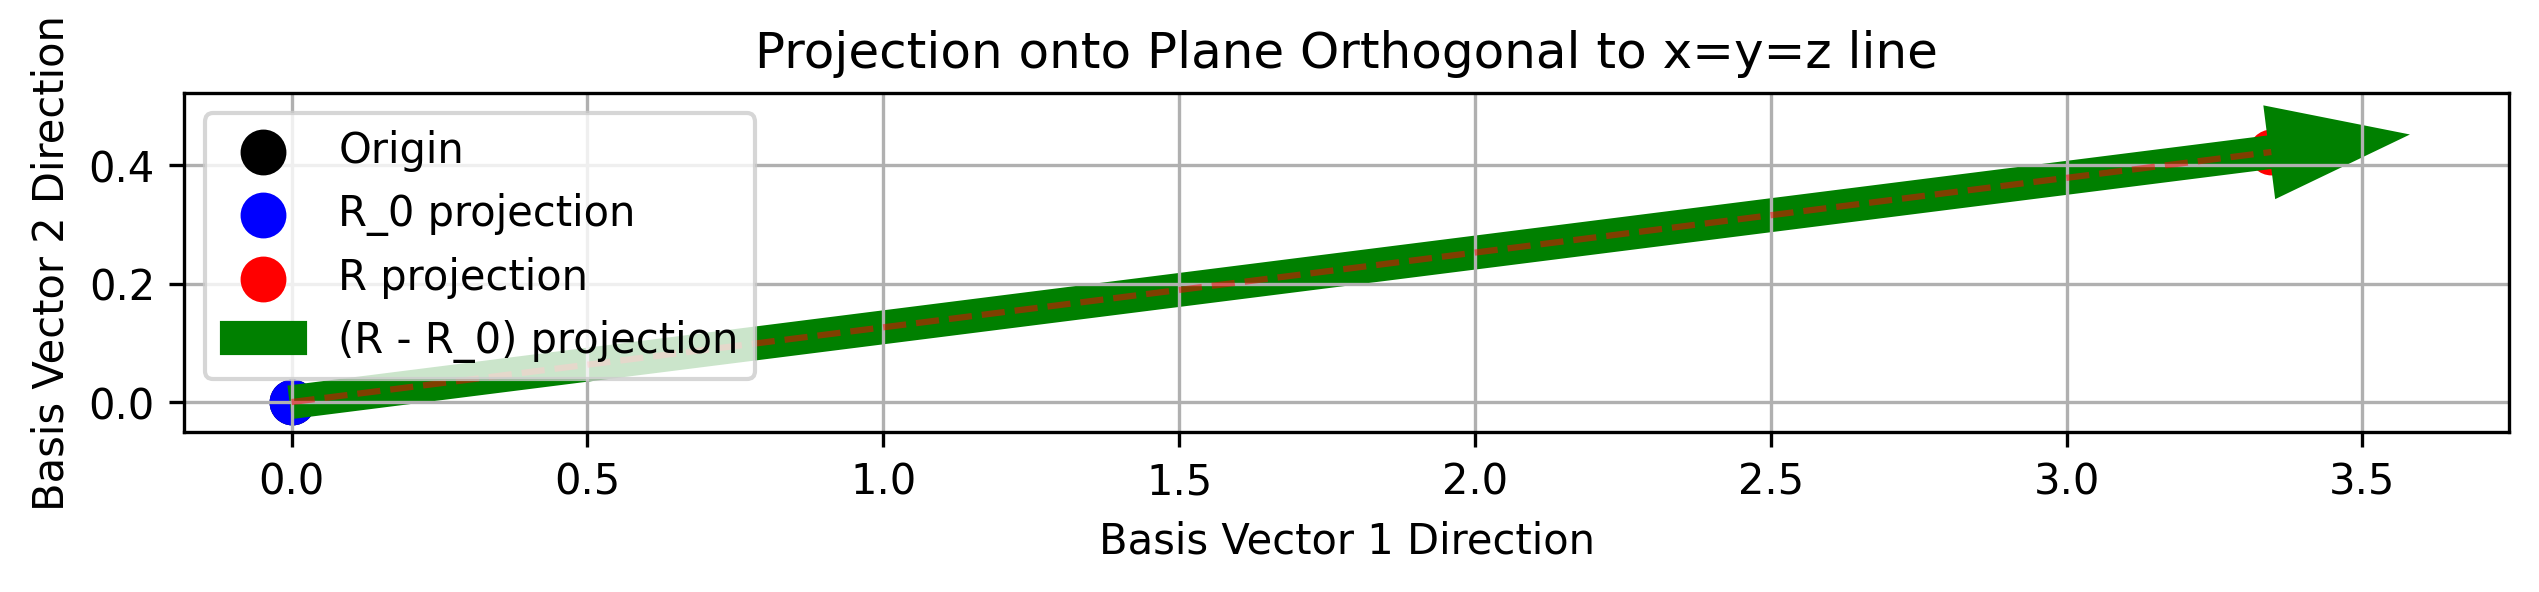
\includegraphics[width=0.8\textwidth]{figures/orthogonality_test/orthogonality_test_2d.png}
    \caption{2D projection onto the plane orthogonal to the x=y=z line}
    \label{fig:orthogonality_test_2d}
\end{figure}

\subsubsection{Circle Orthogonality Test}

A test was conducted to verify that vectors generated by varying $\theta$ from 0 to $2\pi$ form a circle in the plane orthogonal to the x=y=z line. The test used 73 points (5-degree increments) and confirmed that all generated vectors maintain orthogonality to the (1,1,1) direction.

\begin{figure}[H]
    \centering
    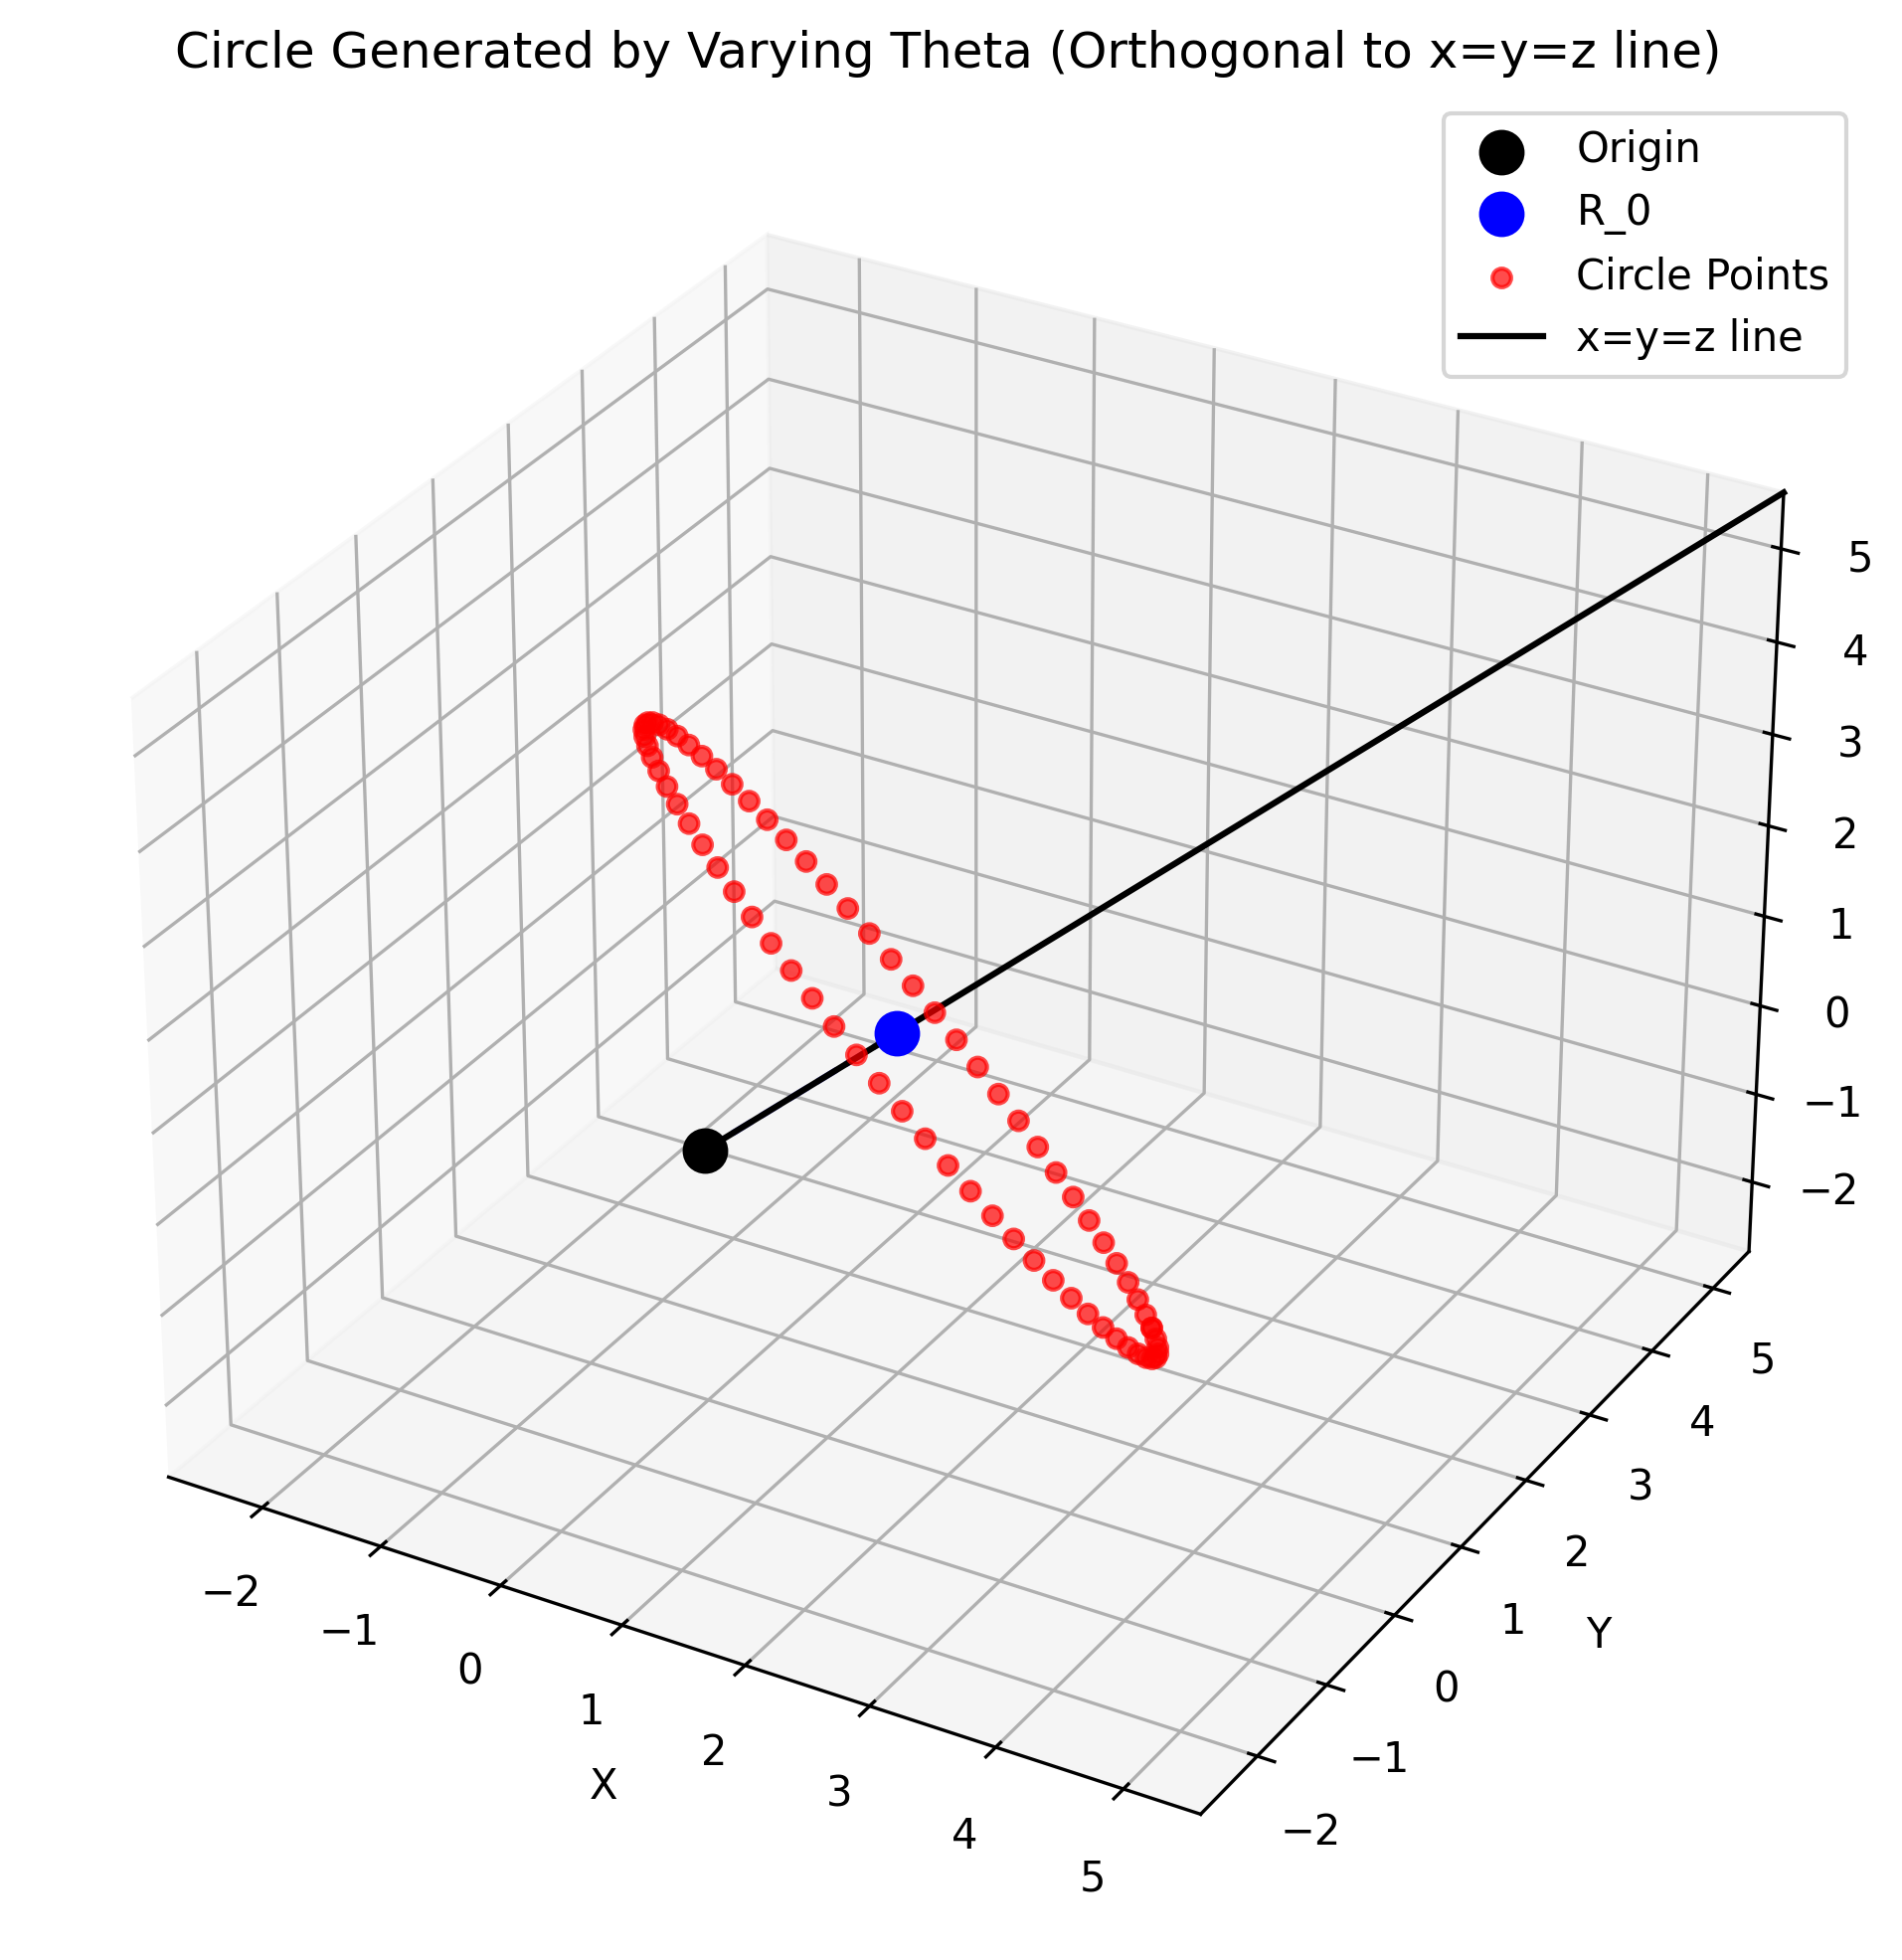
\includegraphics[width=0.8\textwidth]{figures/orthogonality_test/orthogonality_circle_3d.png}
    \caption{3D visualization of the circle formed by vectors orthogonal to the x=y=z line}
    \label{fig:orthogonality_circle_3d}
\end{figure}

\begin{figure}[H]
    \centering
    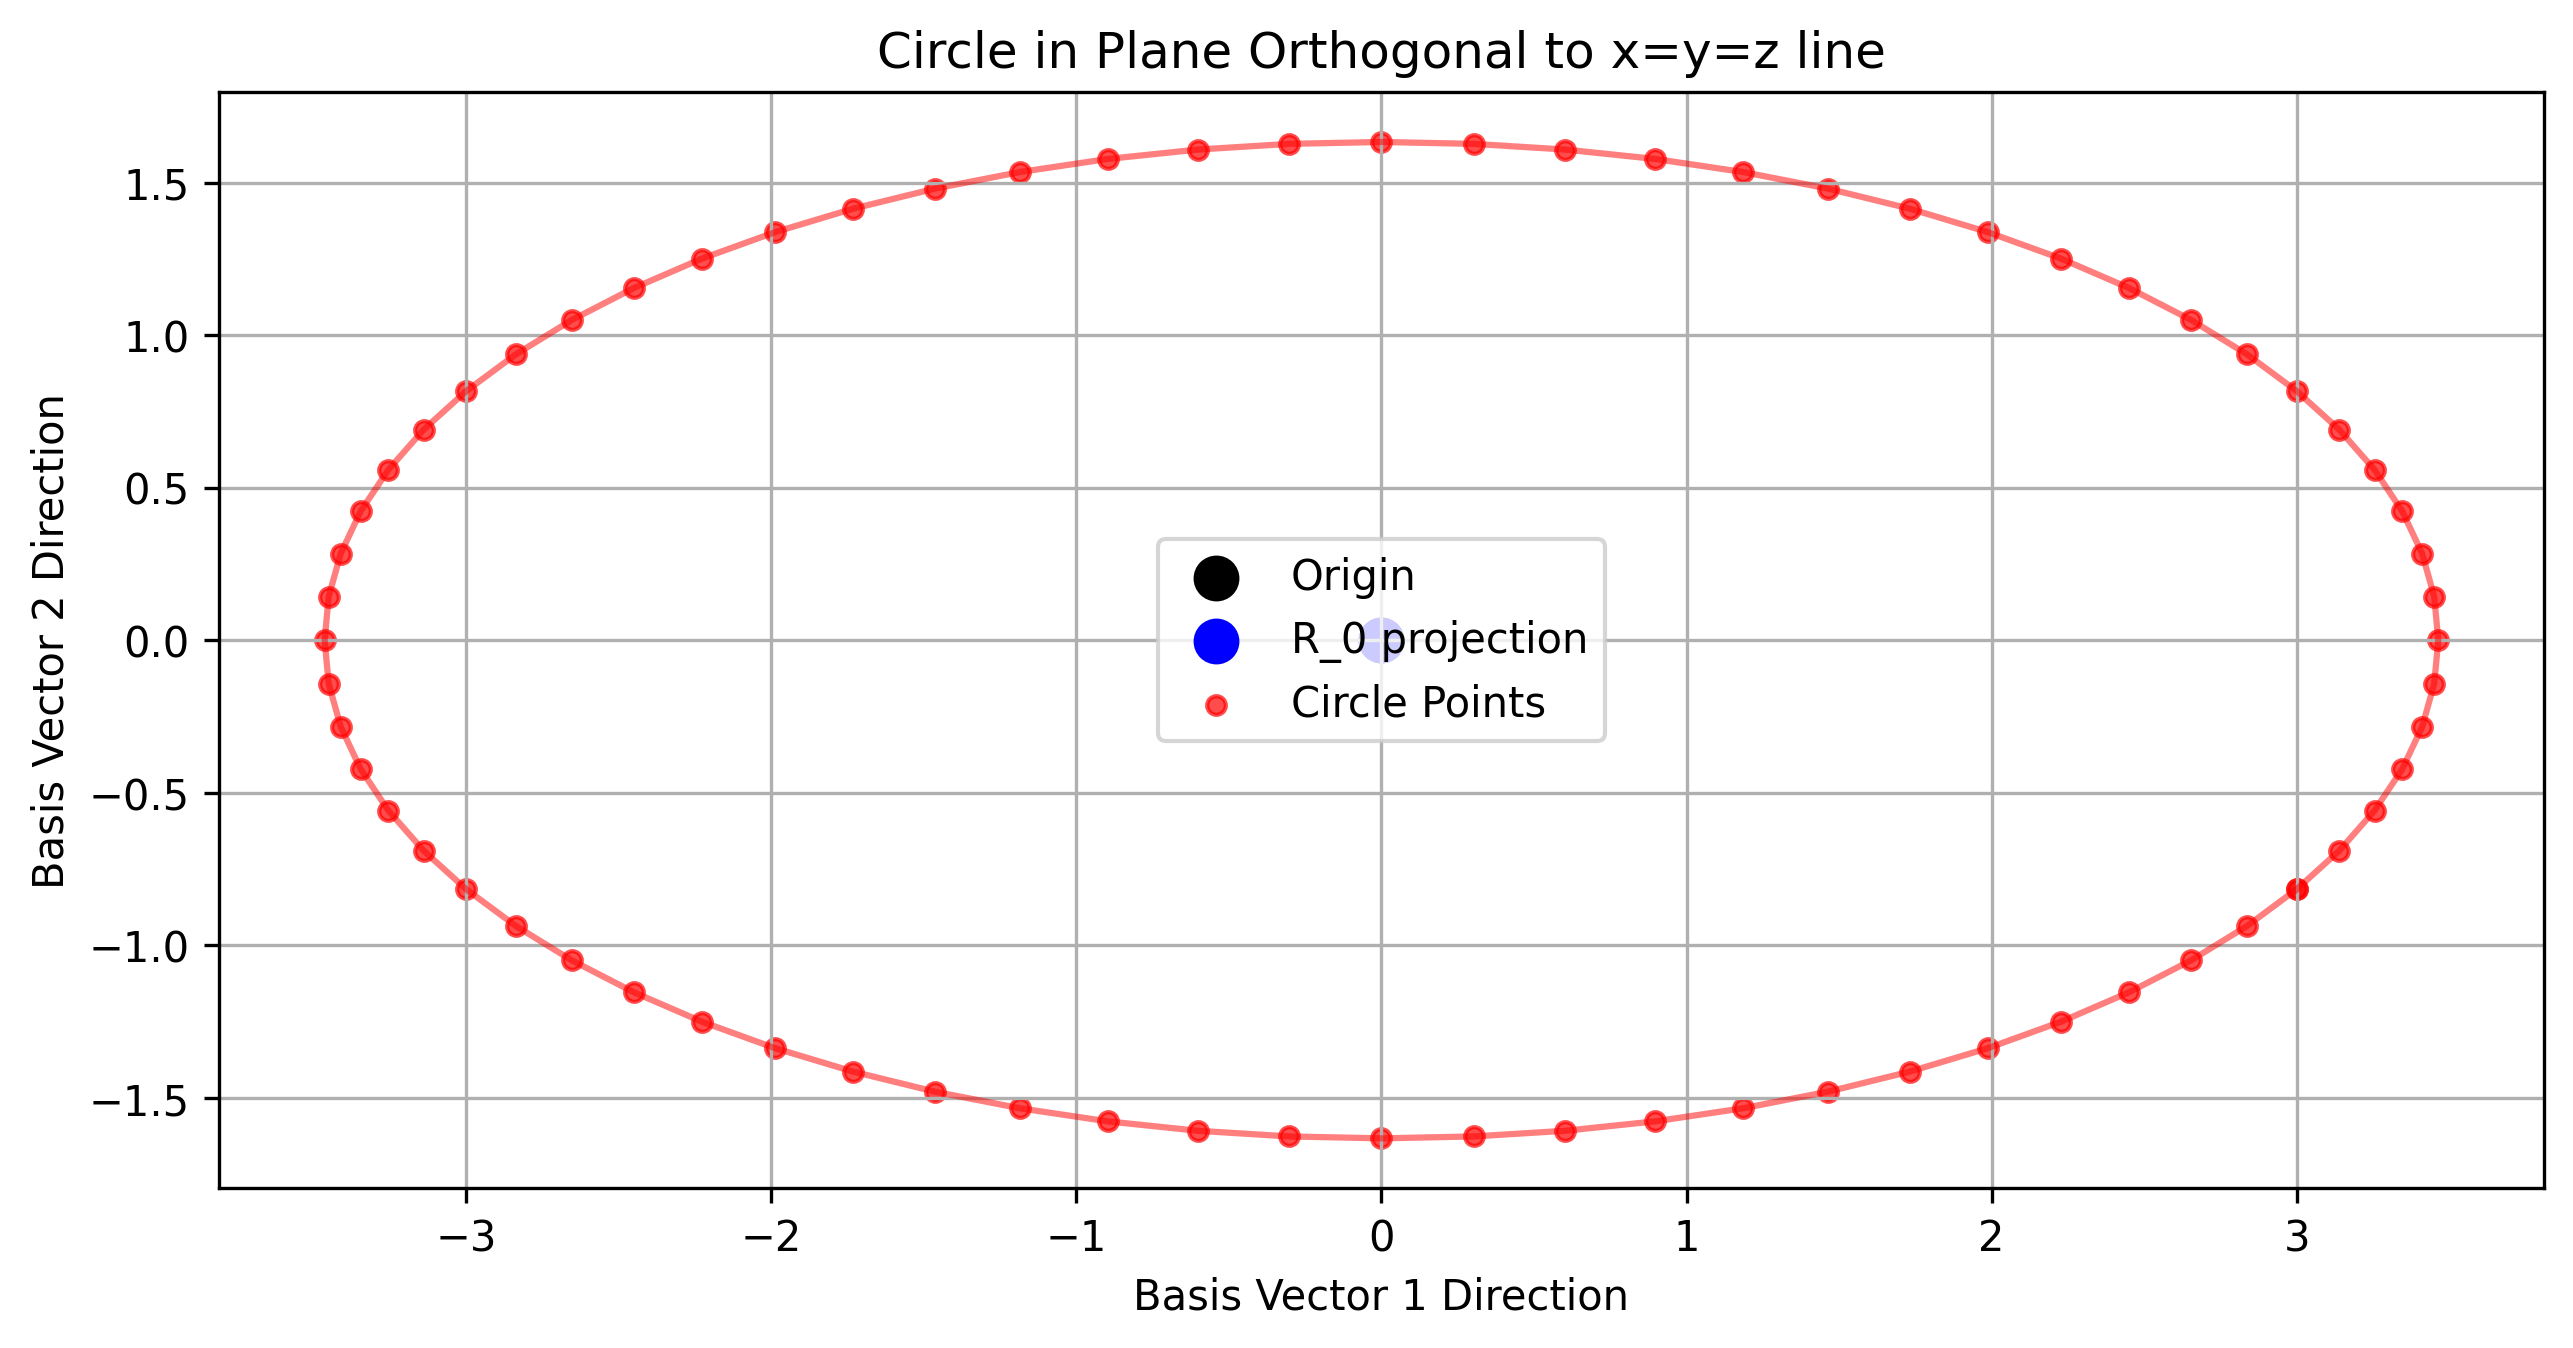
\includegraphics[width=0.8\textwidth]{figures/orthogonality_test/orthogonality_circle_2d.png}
    \caption{2D projection of the circle onto the plane orthogonal to the x=y=z line}
    \label{fig:orthogonality_circle_2d}
\end{figure}

\subsubsection{Comprehensive Circle Visualization}

A comprehensive visualization was created to show the circle from multiple perspectives:

\begin{figure}[H]
    \centering
    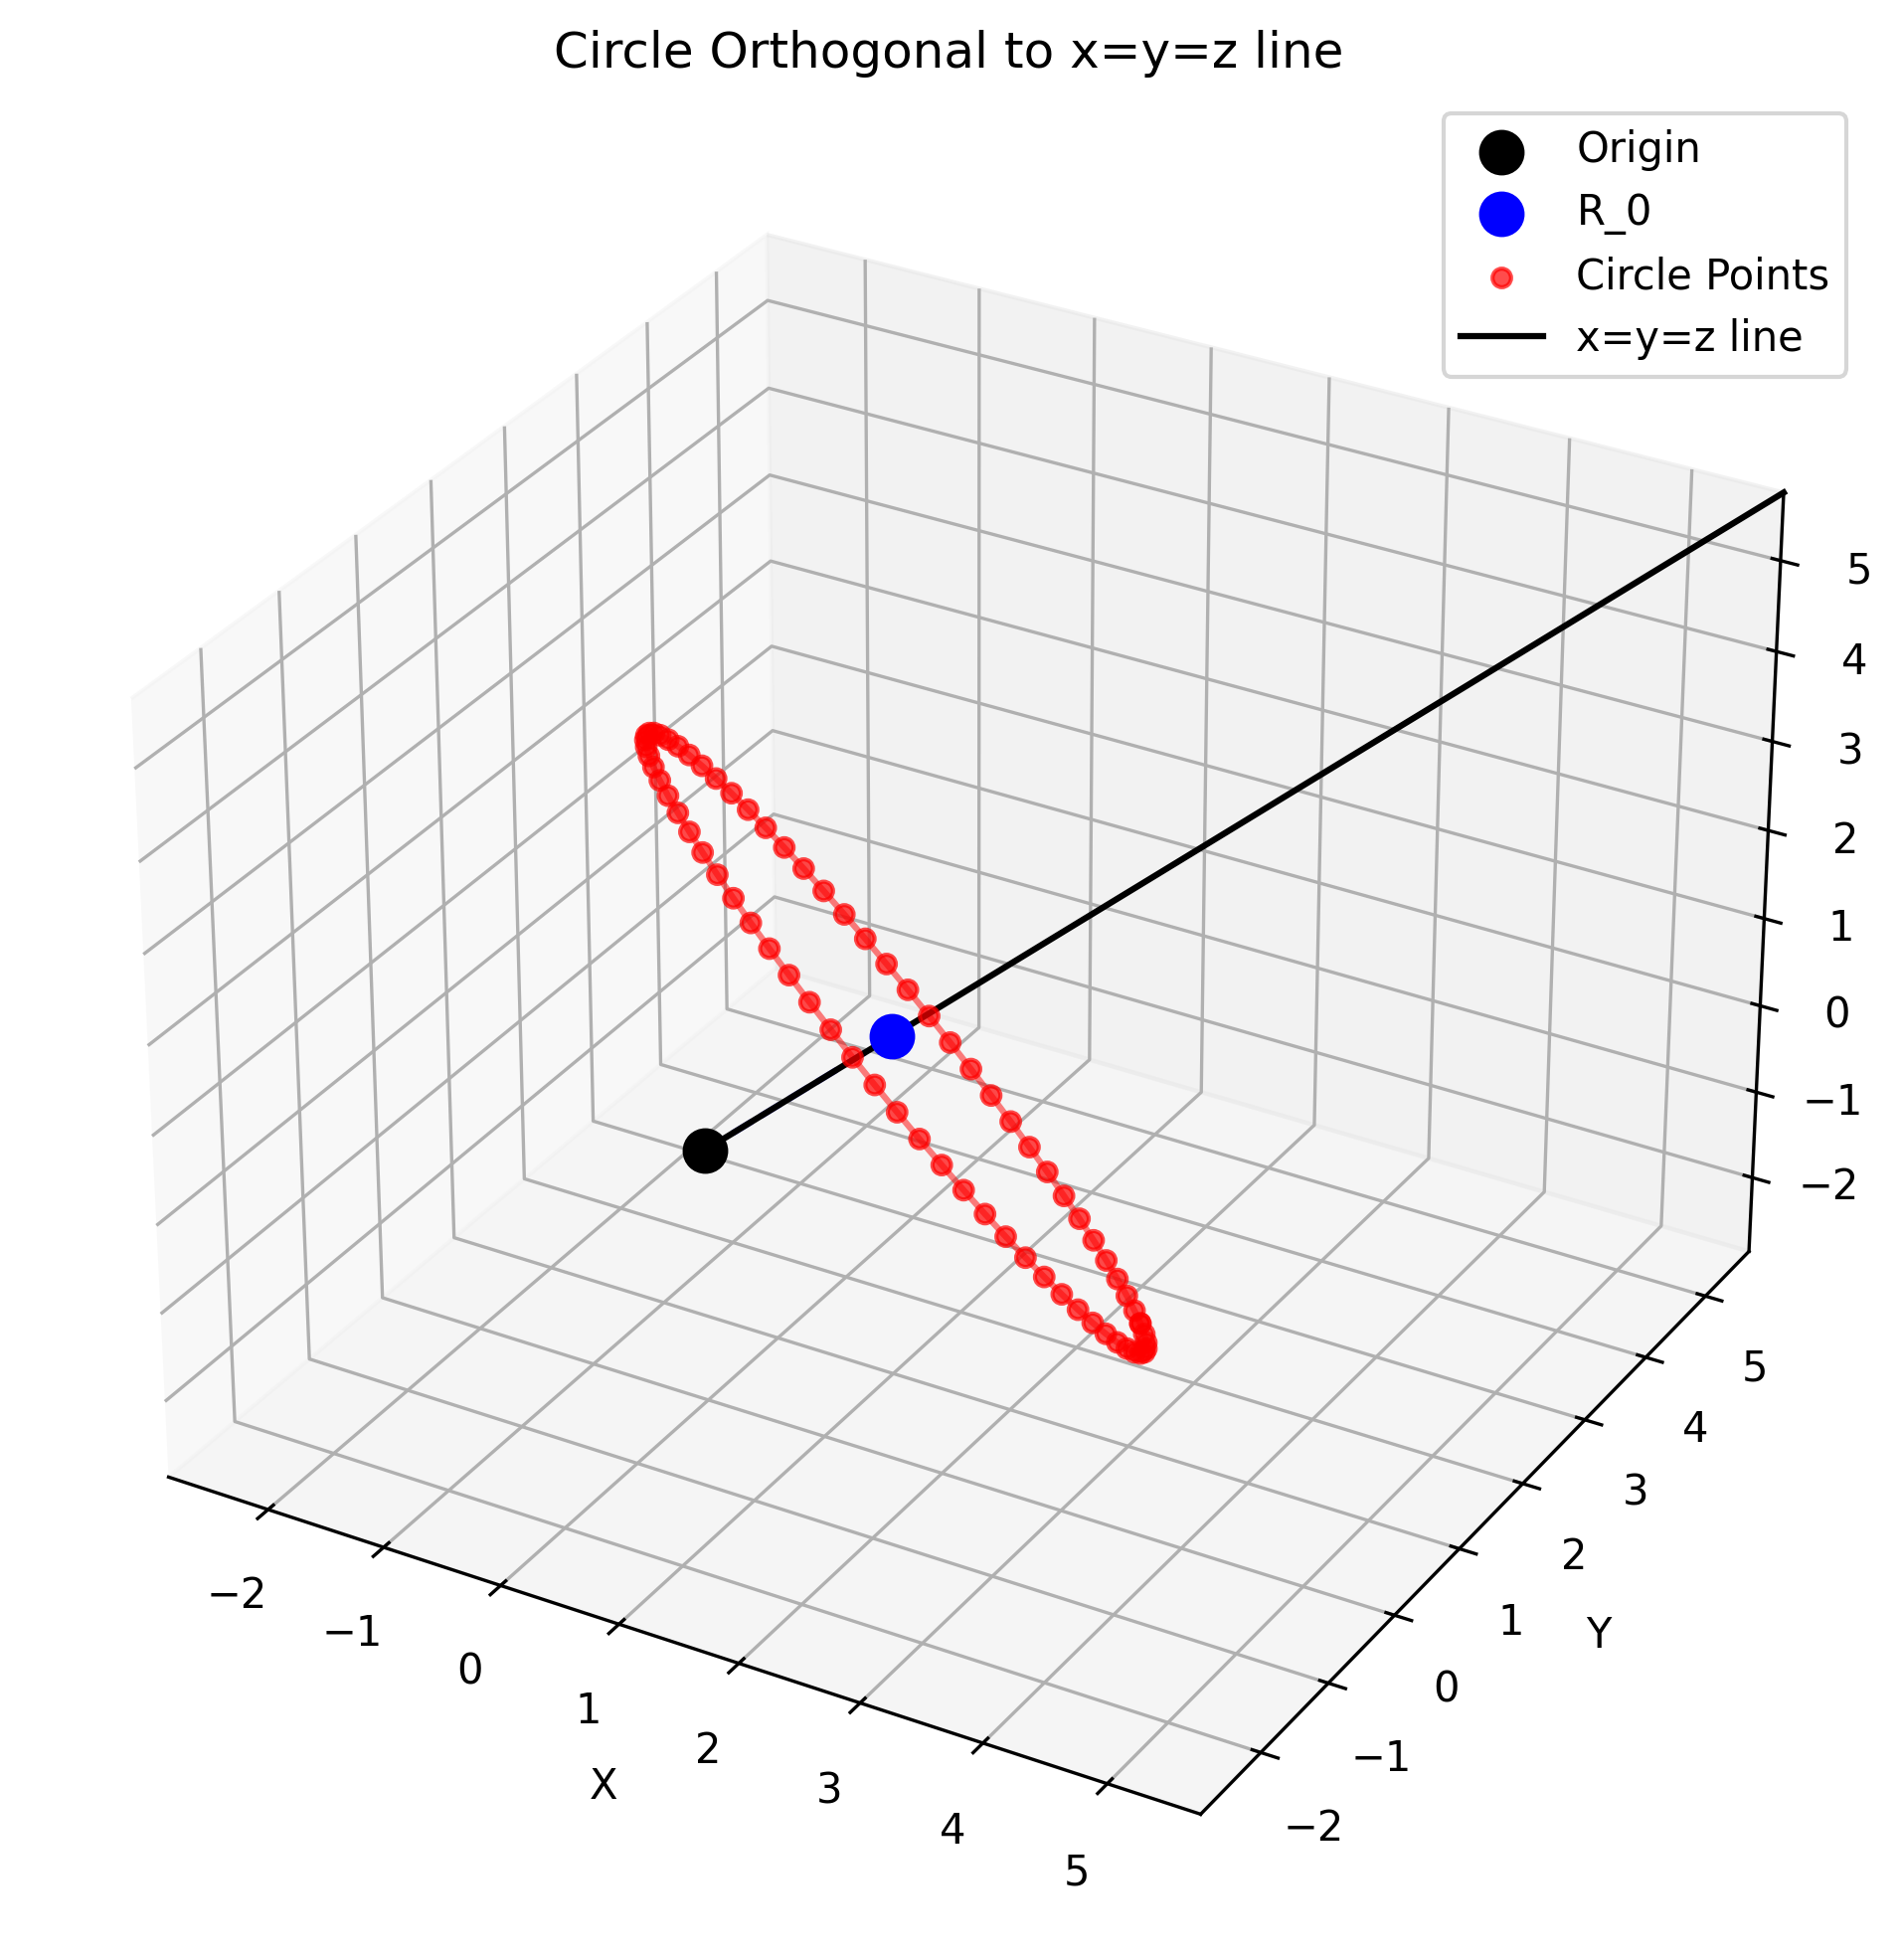
\includegraphics[width=0.8\textwidth]{figures/orthogonality_test/orthogonal_circle_3d.png}
    \caption{3D visualization of the circle orthogonal to the x=y=z line}
    \label{fig:orthogonal_circle_3d}
\end{figure}

\begin{figure}[H]
    \centering
    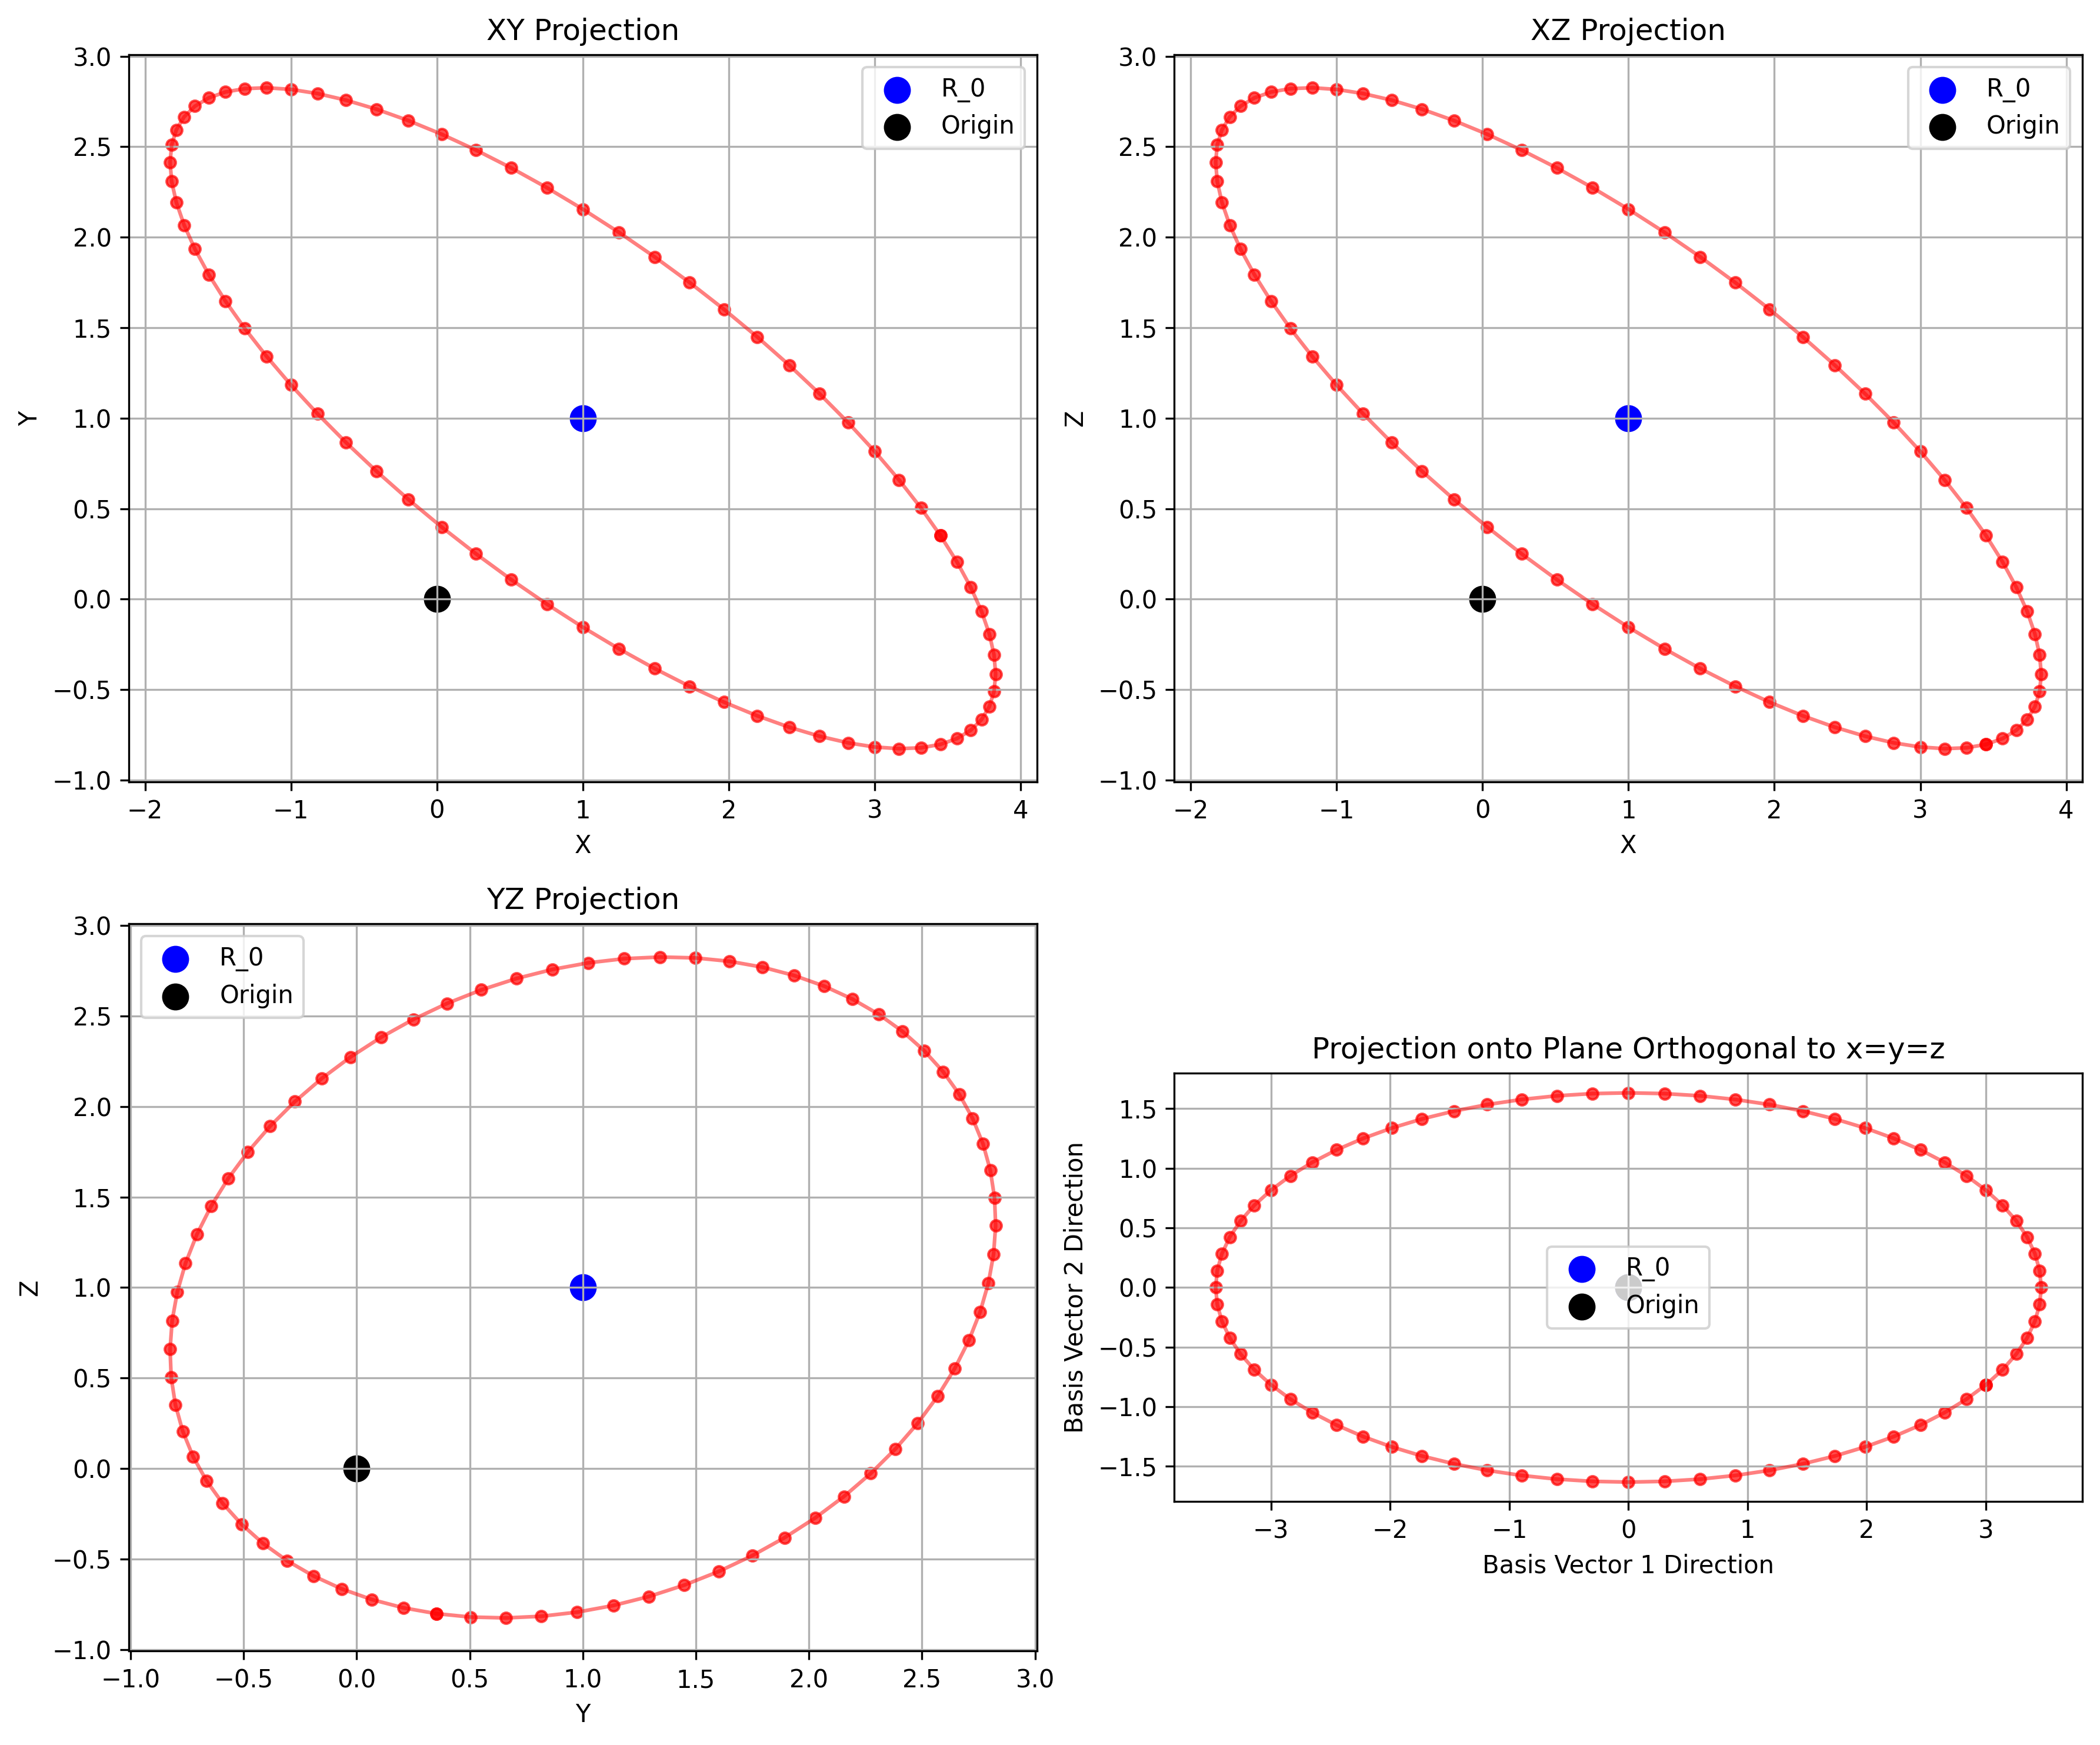
\includegraphics[width=0.8\textwidth]{figures/orthogonality_test/orthogonal_circle_projections.png}
    \caption{Projections of the circle onto different planes, including the plane orthogonal to the x=y=z line (bottom right)}
    \label{fig:orthogonal_circle_projections}
\end{figure}

\subsubsection{Orthogonality Verification Results}

The tests verified orthogonality by calculating the dot product between the displacement vector (R - R\_0) and the normalized (1,1,1) direction:

\begin{itemize}
    \item Maximum dot product across all points: 5.55e-16
    \item Average dot product: 1.39e-16
\end{itemize}

These values are effectively zero (within floating-point precision), confirming that all generated vectors are orthogonal to the x=y=z line.

\subsection{Parameter Effects in Basis Vector Formulation}

The basis vector formulation uses two key parameters to control the generated vectors: the distance parameter $d$ and the angle parameter $\theta$. These parameters interact with the origin vector to produce a wide variety of vector configurations while maintaining orthogonality to the x=y=z line.

\subsubsection{Distance Parameter}

In the basis vector formulation, the distance parameter $d$ appears as a scaling factor in the formula:

\begin{align}
\vec{R} = \vec{R}_0 + d \cdot \cos(\theta) \cdot \sqrt{\frac{2}{3}} \cdot \vec{b}_1 + d \cdot \frac{\cos(\theta)/\sqrt{3} + \sin(\theta)}{\sqrt{2}} \cdot \vec{b}_1 + d \cdot \frac{\sin(\theta) - \cos(\theta)/\sqrt{3}}{\sqrt{2}} \cdot \vec{b}_2 \cdot \sqrt{2}
\end{align}

where $\vec{b}_1 = [1, -1/2, -1/2]$ and $\vec{b}_2 = [0, -1/2, 1/2]$ are the basis vectors orthogonal to the (1,1,1) direction.

This parameter controls the overall scale of the vector displacement from the origin. Larger values of $d$ result in vectors that extend further from the origin, while smaller values produce vectors closer to the origin. The distance parameter affects all components of the vector equally, preserving the directional properties determined by $\theta$ and the orthogonality to the x=y=z line.

\subsubsection{Angle Parameter}

The angle parameter $\theta$ appears in both sine and cosine terms in the basis vector formula. This parameter controls the orientation of the generated vector within the plane orthogonal to the x=y=z line. As $\theta$ varies, the vector traces a circle in the plane orthogonal to the x=y=z line.

\subsubsection{Multiple Perfect Circles with Different Distances}

To illustrate the effect of the distance parameter $d$, we can generate multiple perfect circles with different distance values while keeping the same origin and angle range. Figure \ref{fig:perfect_circle_distance_range} shows perfect orthogonal circles with distances ranging from 0.5 to 3.0 in 0.5 increments, all centered at the origin [0.0, 0.0, 0.0].

\begin{figure}[H]
    \centering
    \includegraphics[width=0.8\textwidth]{../../../perfect_circle_distance_range.png}
    \caption{3D visualization of perfect orthogonal circles with different distance values (d = 0.5 to 3.0)}
    \label{fig:perfect_circle_distance_range}
\end{figure}

\begin{figure}[H]
    \centering
    \includegraphics[width=0.8\textwidth]{../../../perfect_circle_distance_range_projections.png}
    \caption{Projections of the perfect orthogonal circles with different distance values onto different planes}
    \label{fig:perfect_circle_distance_range_projections}
\end{figure}

These figures clearly demonstrate how the distance parameter $d$ controls the radius of the circle in the plane orthogonal to the x=y=z line. All points on each circle remain perfectly orthogonal to the x=y=z line, regardless of the distance value. This property makes the perfect orthogonal circle generation method particularly useful for applications requiring precise control over both orthogonality and distance from the origin.

\subsubsection{Enhanced Visualization Features}

The visualizations incorporate several enhancements for improved clarity and spatial understanding:

\begin{itemize}
    \item \textbf{Color-coded Axes}: The X (red), Y (green), and Z (blue) axes are color-coded for easy identification.
    \item \textbf{Coordinate Labels}: Integer coordinate values are displayed along each axis, color-matched to the axis color.
    \item \textbf{Tick Marks}: Small tick marks are added along each axis for better spatial reference.
    \item \textbf{Data-driven Scaling}: The axis limits are dynamically adjusted based on the actual data points, making the circles more prominent in the visualization.
    \item \textbf{Equal Aspect Ratio}: The 3D plots maintain an equal aspect ratio for accurate spatial representation.
    \item \textbf{Buffer Zones}: Small buffer zones are added around the data points for better visibility.
\end{itemize}

These visualization enhancements significantly improve the clarity of the 3D representations, making it easier to understand the spatial relationships between the circles and their orthogonality to the x=y=z line.

The angle parameter works by controlling the linear combination of the two basis vectors $\vec{b}_1 = [1, -1/2, -1/2]$ and $\vec{b}_2 = [0, -1/2, 1/2]$, which span the plane orthogonal to the (1,1,1) direction. As $\theta$ varies, the vector traces a circular path in this orthogonal plane while maintaining a constant distance from the origin (for fixed $d$). The sine and cosine terms determine the specific linear combination, ensuring that the resulting vector always remains orthogonal to the x=y=z line.

When $\theta$ is varied from 0 to $2\pi$ with a fixed distance parameter, the resulting vectors form a perfect circle in the plane orthogonal to the x=y=z line, as demonstrated in the orthogonality test results. This is fundamentally different from a traditional circle in the XY plane, which is not generally orthogonal to the (1,1,1) direction.

The orthogonality to the x=y=z line is maintained for all values of $\theta$, as verified by the dot product calculations in the orthogonality tests.

\subsubsection{Flexible Parameter Support}

The perfect orthogonal circle generation method supports flexible parameters for customization:

\begin{itemize}
    \item \textbf{Arbitrary Origin}: The circle can be generated around any origin point $\vec{R}_0$, not just the coordinate system origin.
    \item \textbf{Variable Distance}: The distance parameter $d$ can be set to any positive value, controlling the radius of the circle.
    \item \textbf{Theta Range}: The circle can be generated as a complete circle or as a segment by specifying start\_theta and end\_theta parameters.
\end{itemize}

\subsubsection{Parameter Verification Results}

Comprehensive testing with different parameter values confirms the robustness of the implementation:

\begin{table}[H]
    \centering
    \begin{tabular}{|c|c|c|c|}
        \hline
        \textbf{Distance ($d$)} & \textbf{Mean Distance} & \textbf{Std. Dev.} & \textbf{Max Dot Product} \\ \hline
        0.5 & 0.5 & 1.18e-16 & 1.94e-16 \\ \hline
        1.0 & 1.0 & 1.35e-16 & 1.67e-16 \\ \hline
        2.0 & 2.0 & 2.16e-16 & 3.33e-16 \\ \hline
        3.0 & 3.0 & 3.70e-16 & 3.33e-16 \\ \hline
    \end{tabular}
    \caption{Verification results for different distance values}
    \label{tab:distance_verification}
\end{table}

\begin{table}[H]
    \centering
    \begin{tabular}{|c|c|c|c|c|}
        \hline
        \textbf{Theta Range} & \textbf{Mean Distance} & \textbf{Std. Dev.} & \textbf{Max Dot Product} & \textbf{Points} \\ \hline
        $(0, \pi/2)$ & 2.0 & 1.89e-16 & 3.33e-16 & 18 \\ \hline
        $(0, \pi)$ & 2.0 & 2.09e-16 & 3.33e-16 & 18 \\ \hline
        $(\pi/4, 3\pi/4)$ & 2.0 & 2.22e-16 & 4.44e-16 & 18 \\ \hline
        $(0, 2\pi)$ & 2.0 & 2.56e-16 & 3.33e-16 & 18 \\ \hline
    \end{tabular}
    \caption{Verification results for different theta ranges}
    \label{tab:theta_verification}
\end{table}

\begin{figure}[H]
    \centering
    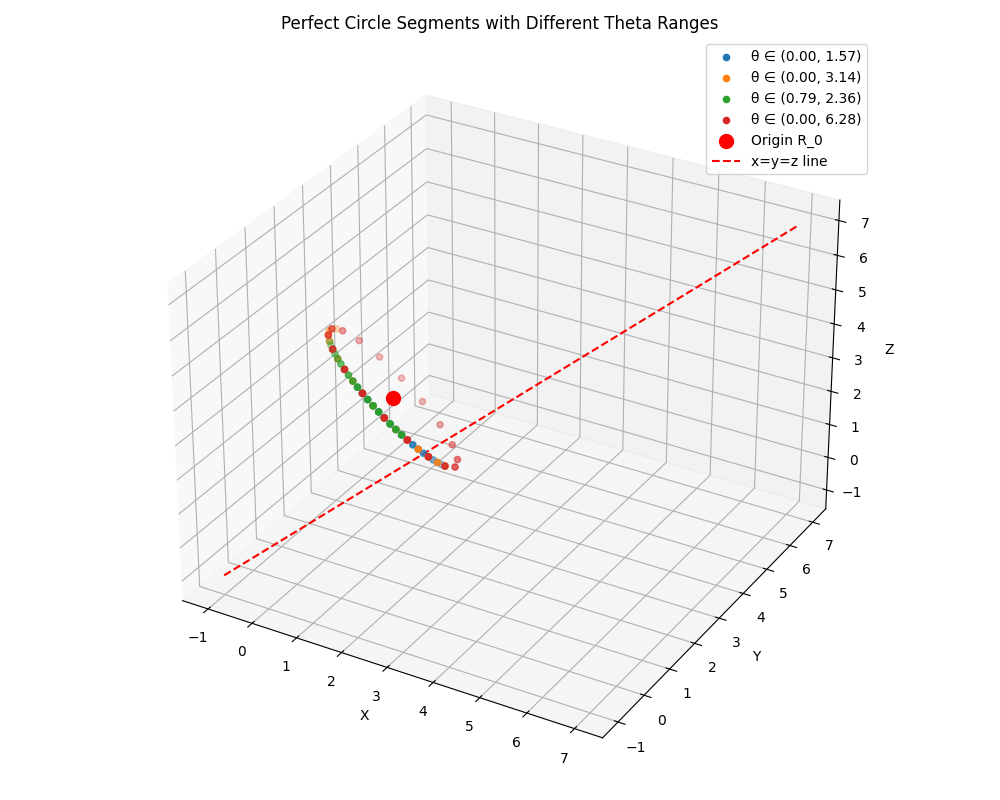
\includegraphics[width=0.8\textwidth]{../../../perfect_circle_tests.png}
    \caption{3D visualization of perfect circles with different distance values and theta ranges}
    \label{fig:perfect_circle_tests}
\end{figure}

These results confirm that the perfect orthogonal circle implementation maintains exact distance from the origin and perfect orthogonality to the (1,1,1) direction across all parameter variations. The standard deviation of distances is effectively zero (within floating-point precision), and the maximum dot product with the (1,1,1) direction is also effectively zero.


\subsection{Summary of Results}

The example results demonstrate that the Generalized Orthogonal Vectors Generator and Visualizer successfully generates and visualizes orthogonal vectors for various configurations. The vectors are confirmed to be orthogonal by calculating their dot products, which are all zero (within numerical precision).

The visualizations show the vectors in both 3D and 2D projections, providing different perspectives on their spatial relationships. The enhanced visualization features, including color-coded axes, coordinate labels, and data-driven scaling, significantly improve the clarity of the representations and make it easier to understand the spatial relationships between the vectors.

The effects of the distance parameter, angle parameter, and origin on the vector system are clearly demonstrated through the various examples, with the improved visualizations making these relationships more apparent.
